\chapter{Vorgehen}
\label{ch_vorgehen} 

Das Ziel ist die Entwicklung eines Prototypen aus dem bestehenden Modell der Projektarbeit von \cite{PA_bicycle}. Die Vorgehensschritte sind in der untenstehenden Auflistung abgebildet. Sie bilden die Struktur dieses Kapitels. Die Definition der konkreten Schritte geschah in Absprache mit Prof. Dr. M. Meli und dem Resarch Assitenten Herr Dario Dünar vom Instiut of Embedded Systems (InES). Auf der CD finden sich die Sitzungsprotokolle über den aktuellen Entwicklungsstand, die offenen Fragen und die Entscheidungen.

\subsubsection*{Liste der Arbeitsschritte}
\label{liste} 

\begin{enumerate}
  \item Inbetriebnahme Machbarkeitsstudie  
  \item Hardware entwickeln  
  \item Inbetriebnahme Prototyp      
  \item Energy und Power Management
  \item Entwickeln einer BLE-Applikation       
 \end{enumerate}  

Die sprachliche Unterscheidung von Energy - und Power Management entspricht der Unterscheidung zweier \glqq Management-Teilen\grqq\medskip im Prototypen: Das Endprodukt regelt an zwei Stellen auf unterschiedliche Art die zur Verfügung stehende Energie. Der Begriff Energy Management wird in dieser Arbeit für das Sammeln und Weiterleiten von Energie über eine Hardwareimplementation gebraucht. Der Begriff Power Management wird für die Softwareimplementation gebraucht. Diese regelt, dass die zur Verfügung gestellte Energie nicht sofort verbraucht wird. Die sprachliche Trennung ist künstlich, denn in der Umsetzung spielen Hard- und Softwareregelung Hand in Hand. Die sprachliche Unterscheidung dient der Lesbarkeit und bezeichnet keinen physikalischen Unterschied.
 
 
 % 1---------------------------------------------------------------------------
 %------------------------------------------------------------------------------
  
 
\section{Inbetriebnahme Machbarkeitsstudie}\label{v_inbetriebnahme} 

      
Ziel der Inbetriebnahme des Aufbaus der vorangehenden Arbeit \cite{PA_bicycle} ist es, zu definieren, welche Funktionalitäten verbessert werden sollen. Zur Orientierung werden im ersten Unterkapitel \ref{fb} die Funktionsblöcke und deren Aufgaben festgehalten. Danach wird das Verhalten der Vorgängermodells in Unterkapitel \ref{verhalten} ausgemessen. Aus der Analyse entsteht die in Unterkapitel \ref{optimierung} aufgelistete erste Optimierungsliste. Als letztes folgt eine Vertiefung in das auffällige Verhalten des Eingangssignals in Unterkapitel \ref{auffaellig}. Dieser Exkurs hat Ursache in der Begegnung mit  Ives Théoduloz von EM MicroElectronic. Er entwickelte den in dieser Arbeit verwendete EM8500-Chip mit und wies uns auf den auffälligen Signalverlauf des Harvester-Eingangssignals (siehe Abbildung \ref{spannungMachbarkeit}) hin. Dieses Signal wurde deshalb bei der Inbetriebnahme eigens getestet, was im letzten Unterkapitel dokumentiert ist.
      
\subsection{Funktionsblöcke}\label{fb} 

Der Bicycle Computer besteht aus vier Funktionsblöcken, die in der Abbildung \ref{funktionsdiagramm_bild} dargestellt sind. Der erste Funktionsblock ist der Harvester (siehe 1) in der Abbildung \ref{funktionsdiagramm_bild}). Die Aufgaben des Harvesters ist es Energie zu Ernten und dem nächsten Funktionsblock (Nummer 2) in der Abbildung  \ref{funktionsdiagramm_bild} zur Verfügung zu stellen. Der zweite Funktionsblock wird als Energy Management-Teil in der Arbeit bezeichnet. Die Aufgabe des zweiten Blocks ist es, Energie zu Sammeln und kontrolliert an die Verbrauchsstelle freizuschalten. Detaillierte Informationen finden sich in den Theoretischen Grundlagen im Unterkapitel \ref{t_energy_management}. Der dritte Funktionsblock ist der Ort, an dem die Energie verbraucht wird. In dieser Arbeit dient die Energie dem Betreiben von Sensoren und dem versenden derer Daten. Dies wird auf dem Sensortag (siehe Anhang \ref{anhang_sensortag}) umgesetzt. Der Grund dafür wird in der Einleitung des Kapitels \label{t_power_management} dargelegt. Der letzte Funktionsblock bezeichnet das Ziel, das Erhalten von Sensordaten in einer Applikation.  

\begin{figure}[ht]
   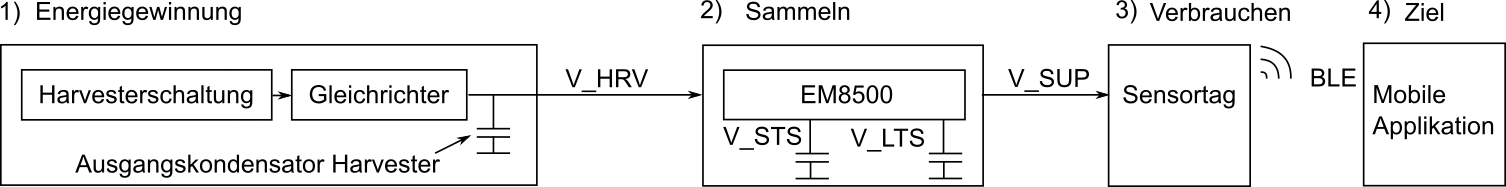
\includegraphics[width=1\textwidth]{3Vorgehen/imag/Blockdiagramm.png}
   \caption{Funktionsblöcke Bicycle Computer}
   \label{funktionsdiagramm_bild} 
\end{figure}

Den Funktionsblöcke sind Spannungsbezeichnungen sowie Kondensatoren beigefügt. Dies, weil bei der Beschreibung des Verhaltens des Vorgängermodells, diese Spannungslevel für die Funktionsbeurteilung wichtig werden. Die nachfolgende Legende beschreibt die Beschriftung näher.

\subsubsection*{Legende Abbildung \ref{funktionsdiagramm_bild}}
\label{legende}

\begin{tabbing}
    Bezeichnung \quad\= Beschreibung\\[0.8ex]
    V\_HRV \> Ausgangspannung Harvesterquelle, Eingangsspannung Energy Management\\
    V\_STS\> Spannung am STS--Kondensator (Primärspeicher)\\
    V\_LTS\> Spannung am LTS--Kondensator (Sekundärspeicher)\\
    V\_SUP\> Ausgangsspannung Energy Managment, Eingangsspannung Sensortag\\
    BLE \> Senden der Daten per Bluetooth Low Energy (siehe \ref{t_ble} \\
\end{tabbing}   

\todo{Header Tabelle (Bezeichnung, Beschreibung) weg } 

\subsection{Verhalten des Vorgängermodells}\label{verhalten} 

Die Inbetriebnahme bestätigte das in der Dokumentation \cite{PA_bicycle} beschriebene Verhalten. Die Abbildung \ref{spannungMachbarkeit} zeigt den zeitlichen Verlauf der Energiestände zwischen den Funktionsblöcken (siehe Abbildung \ref{funktionsdiagramm_bild} und an den Speicherelementen. Die Legende zur Abbildung  \ref{spannungMachbarkeit} erklärt die Signale.

\begin{figure}[ht]
    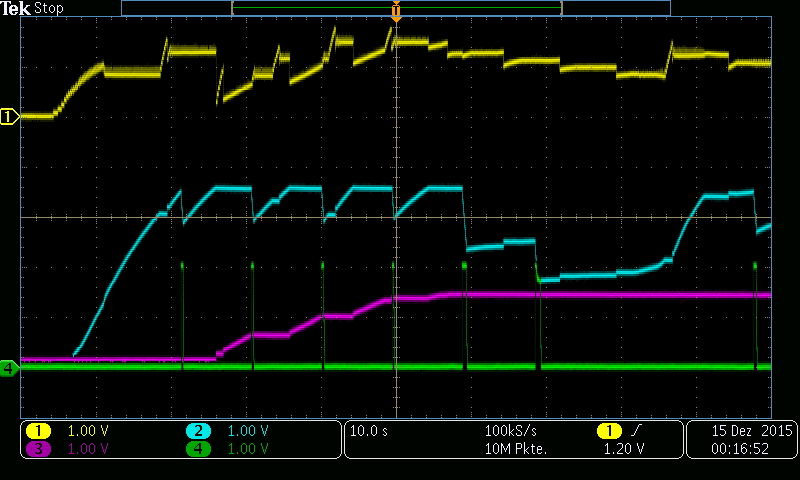
\includegraphics[width=0.5\textwidth]{3Vorgehen/imag/messungPA.png}
    \caption{Spannungswerte Modell der Machbarkeitsstudie}\label{spannungMachbarkeit} 
\end{figure}

\subsubsection*{Legende Abbildung \ref{spannungMachbarkeit} }
\begin{tabbing}
    Channel\quad\= Farbe\quad\= Beschreibung\\[0.8ex]
    CH1\> gelb\> Spannungsverlauf V\_HRV\\
    CH2\> blau\> Spannungsverlauf am STS--Kondensator\\
    CH3\> violet\> Spannungsverlauf am LTS--Kondensator\\
    CH4\> grün\> Ausgangsspannung nach Energy Management\\
     \>  \>      Eingangsspannung Sensorttag
\end{tabbing}    

Im Folgenden werden die einzelnen Spannungsverläufe chronologisch der Kanalnummer nach analysiert. Kanal 1 spiegelt die Spannung am Harvesterausgang wieder (V\_HRV). Gemäss Theorie \ref{eingangsspannung} bzw. gemäss Datenblatt des EM8500 ist der EM8500-Chip für ein DC-Signal ausgelegt. Er geht von einem regelmässigen Eingangssignal aus und regelt die Spannung auf den MPPT. Diese Regelung sollte wie in Abbildung \ref{RegelungSpannung} aussehen. Das reale Signal entspricht nicht diesem Verhalten. Die Regelung ist abrupt und überspringt mehrere Spannungslevel. Der Ursache für die schlechte Regelung soll nachgegangen werden.

Kanal 2, blau, gibt den Spannungsverlauf am Hauptspeicher, dem Primärspeicher, der in der im Datenblatt von EM8500 STS heisst, wieder. Das Energy Management des Vorgängermodells setzt den Schwellwert für den Primärspeicher (STS) mit 3.6 V hoch (Details zu den Schwellwerten im Kapitel Theoretische Grundlagen \ref{t_energy_management}). Der hohe Wert erklärt durch das Ziel, genug Energie für ein konstantes Paketversenden zu haben. Dies gelingt für fünf BLE-Pakete. Danach reicht die Energie nicht mehr aus. V\_SUP, grünes Signal, wird nicht mehr gespiesen. Nach 30 s ohne Pakete senden ist wieder genug Energie gespeichert, für weitere 5 Datenpakete.

In der Auswertung viel uns auf, dass dieser Signalverlauf nur bei einer Geschwindigkeit 45 km/h möglich ist. Die Speicherkapazität von 470 $\mu$F und ein Schwellwert der Spannung von 3.6 V ist mit normaler Geschwindigkeit (10 km/h) nach 30 min nicht zu erreichen. Fährt man rund 45 km/h so erhält man die in der Abbildung gezeigte Ladezeit von rund 25 s. Eine exakte Geschwindigkeitsmessung ist zu Beginn der Arbeit nicht möglich. Das Rad wird von Hand gedreht und mit einem Metronom wird die Umdrehungsgeschwindigkeit vorgegeben. Bei einem Radumfang von 2.04 m und einer Zeitdifferenz von 160 ms zwischen den Reed-Inpulsen, ergibt die Geschwindigkeit von 45 km/h. Da diese Messmethode über längere Zeit nicht sehr genau ist, bestand eine der Aufgabe nach der Inbetriebnahme im Organisieren eines Messaufbaus. Dieser professionellere Messaufbau wird im Anhang \ref{messaufbau} beschrieben.


Kanal 3, das pinkige Signal, zeigt die Spannung am Long Time Speicher. Die Inbetriebnahme zeigt, dass sich der LTS lädt. Es erstaunt jedoch, dass seine geerntete Energie nicht verwendet wird. Der Spannungswert von LTS geht nie herunter.
Die Vermutung ist, dass der eingestellte Schwellwert für den Bezug von Energie von LTS \ref{energiespeisung_lts} nicht stimmt.

Kanal 4, das grüne Signal, zeigt, die Speisung des Sensortags. In Modell der Projektarbeit steuert der Microkontroller des Sensortags den Verbraucht. Alle 10 s wacht das System auf, bezieht Energie vom EM8500-Ausgang für das Senden eines Paketes und geht dann wieder schlafen. Das Aufwachintervall ist fix.


\subsection{Optimierungsliste}\label{optimierung} 

\todo{ Ev. Texbausteine von oben hier hin}

Aus den Messungen der Inbetriebnahme konkretisierten sich die generellen Aufgaben, die in der ersten Liste der Arbeitsschritte zu Beginn des Vorgehens  beschrieben wurden. Folgende vier Punkte sollen durch den Prototypen verbessert werden: 

\begin{itemize}
     \item Der Verlauf des Harvester-Eingangs wechselt abrupt. Der Eingang soll besser geregelt werden. 
     \item Das Laden des Primärspeichers von 470 $\mu$F in 25 s benötigt es eine Geschwindigkeit von mehr als 60 km/h.  Die Harvesterschaltung soll so weiterentwickelt werden, dass bei 10 km/h genug Energie zum Senden von BLE-Paketen besteht.    
     \item Das zweite Speicherelement, der LTS, entlädt sich nicht. Dadurch kann seine Energie nicht verwendet werden. Die Schwellwerte am EM8500 und ev. die Kondensatorenwerte sollen so angepasst werden, dass sich der zweite Kondensator entlädt
     \item Die Energie wird statisch nach einem fixen Zeitintervall von 10 s genutzt. Das Zeitintervall soll der Geschwindigkeit angepasst werden. Bei höherer Geschwindigkeit soll das Intervall kürzer werden.
\end{itemize} 


Im Resultatsteil Kapitel \ref{ch_resultat} werden die Fortschritte in diesen vier Punkten ausgewiesen.

\subsection{Vertiefung in auffälliges Verhalten des Harvestereingangs}\label{auffaellig} 

Herr Ives Théoduloz hatte uns im Rahmen eines Besuchs auf die Problematik, einer zu grossen Kapazität am Eingang des EM-Chips, hingewiesen. Laut seiner Aussage sollte der Kondensator am Eingang des EM-Chips, bzw. dem Ausgang des Harvesters am besten kleiner sein als 4.7 $\mu$F. Bisher wurde im Aufbau der Machbarkeitsstudie ein Kondensator mit 470 $\mu$F verwendet, Herr Ivex Théoduloz meinte, dass dieser Kondensator viel zu gross sei und dass die Regelung am Eingang des EM-Chips möglicherweise nicht richtig funktionieren würde. Daher wurde dieses Problem näher untersucht und in mehreren Schritten optimiert.

Im ersten Schritt wurde der Kondensator verkleinert, bis die Rippelspannung noch annehmbar war. Die Rippelspannung bei dem bestehenden Kondensator von 470 $\mu$F beträgt ca. 10 mVpp. Die Rippelspannung bei einer Kapazität von 47 $\mu$F beträgt bereits ca. 40 mVpp, jedoch ist die Rippelspannung noch in einem Bereich der annehmbar scheint. Bei einer Kapazität von 10 $\mu$F liegt die Rippelspannung von ca. 500 mVpp, dies ist nicht mehr akzeptabel. Die Abbildung \ref{47uF_mit_Limiter_AC} veranschaulicht die Rippelspannung von einem Kondensator mit 47 $\mu$F, die Abbildung \ref{10uF_mit_Limiter_DC} zeigt die Rippelspannung über einem Kondensator von 10 $\mu$F.

\begin{figure}[ht]
    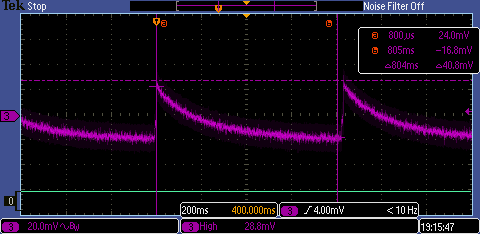
\includegraphics{3Vorgehen/imag/47uF_mit_Limiter_AC.PNG}
    \caption{Rippelspannung über dem 47 $\mu$F Kondensator}
	\label{47uF_mit_Limiter_AC} 
\end{figure}

\begin{figure}[ht]
    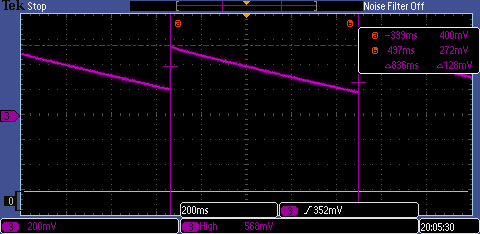
\includegraphics{3Vorgehen/imag/10uF_mit_Limiter_DC.PNG}
    \caption{Rippelspannung über dem 10 $\mu$F Kondensator}
	\label{10uF_mit_Limiter_DC} 
\end{figure}

Jedoch muss auch kritischer Blick auf die Spannung am Harvesterausgang geworfen werden, wenn dieser Ausgang mit dem EM-Chip belastet wird. Es kann beobachtet werden, dass der Eingang des EM-Chips kein konstantes Spannungslevel (siehe Abbildung x) erhält. 

\begin{figure}[ht]
    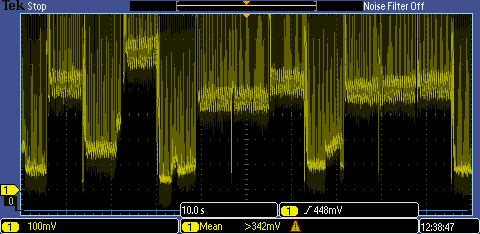
\includegraphics{3Vorgehen/imag/VCC_47uF_15kmh_Periode.PNG}
    \caption{Spannung am EM8500-Eingang über einem 47 $\mu$F Kondensator}
	\label{VCC_47uF_15kmh_Periode} 
\end{figure}

Problematisch ist, dass die Spannung wiederholt unter die 0.3 V Grenze fällt, bei einer Spannung von 0.3 V kann keine Energie gespeichert werden. Die Regelung am Eingang des EM-Chips kommt mit der anliegenden Rippelspannung nicht klar. Die Rippelspannung muss verringert werden, bzw. die Kapazität am Ausgang des Harvesters muss erhöht werden. 

Das Problem ist, dass durch den Rippel die periodische Open Loop Spannungsmessung keine korrekten Messwerte erhält. Sobald die Last vom Harvesterausgang abgehängt wird, steigt die Spannung über dem Kondensator, jedoch wird die Open Loop Spannung bei einer grossen Kapazität nicht erreicht, da die Zeit, bis der Kondensator komplett geladen ist, sehr gross ist. Jedoch bedeutet eine niedrige Kapazität, dass die Rippelspannung relativ hoch ist und je nach Zeitpunkt der Open Loop Messung eine andere Spannung am Kondensator ergibt und die Spannung am Kondensator steigt bei jeder Messung auf ein anderes Spannungslevel.

Es musste ein Kompromiss gefunden werden, so dass die Spannung am Eingang des EM-Chips auf ein konstantes Level geregelt werden kann. Der Kondensator sollte nicht zu klein sein, damit der Rippel nicht zu gross wird. Andererseits darf der Kondensator nicht zu gross sein, da ansonsten die Open Loop Messung keine richtigen Werte liefert. Der Kompromiss stellt der 100 $\mu$F Kondensator dar, bei diesem ist die Spannung am Eingang relativ konstant und es kann damit gearbeitet werden (siehe Abbildung \ref{VCC_100uF_15kmh_Periode}).

\begin{figure}[ht]
    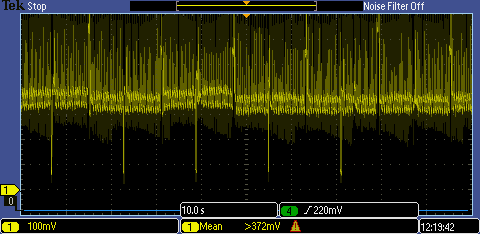
\includegraphics{3Vorgehen/imag/VCC_100uF_15kmh_Periode.PNG}
    \caption{Spannung am EM8500-Eingang über einem 100 $\mu$F Kondensator}
	\label{VCC_100uF_15kmh_Periode} 
\end{figure}

%Text aus Einleitung: Für Argumentation. (Als letztes folgt eine Vertiefung in das auffällige Verhalten des Eingangssignals in Unterkapitel \ref{auffaellig}. Dieser Exkurs hat Ursache in der Begegnung mit  Ives Théoduloz von EM MicroElectronic. Er entwickelte den in dieser Arbeit verwendete EM8500-Chip mit und wies uns auf den auffälligen Signalverlauf des Harvester-Eingangssingals (siehe Abbildung \ref{spannungMachbarkeit}) hin. Dieses Signal wurde deshalb bei der Inbetriebnahme eigens getestet, was im 
%
%??????  .... folgte.) Hier ist nun dieser erwähnte Text.
%
%Vorschlag Katrin:
%Die auffällige Regelung des Harvesterinputs wurd Ives Théoduloz gezeigt. 
%
%Gemäss Ives Théoduloz sollten Kondensatoren der Harvesterschaltung im Bereich von 4.7 $\mu$F liegen, sodass die Energiemanagementschaltung ordnungsgemäss funktioniert.  
%
%
%In der Machbarkeitsstudie ist nach dem Gleichrichter ein Kondensator von 470 $\mu$F nachgeschaltet. Dieser glättet die Spannungspulse nach dem Gleichrichter zu einer DC-ähnlichen Spannung mit Rippeln.
%
%Aus diesem Grund wird die Rippelspannung am Ausgangs der Harvesterschaltung mit kleineren Kondensatoren gemessen. Das Messprotokoll befindet sich im Anhang.
%
%\subsubsection{Ausmessen der Auswirkung des Ausgangskondensators}
%\todo{auf Messprotokoll verweisen}
%
%Mit einem Kondensator von 470 $\mu$F wird die Ausgangsspannung der Harvesterspannung fast rippelfrei. Die Rippelspannung beträgt 3.2 mV (siehe Abbildung \ref{kond470uF}).
%
%\begin{figure}[ht]
%    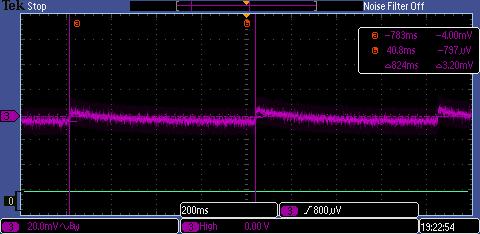
\includegraphics[width=15cm]{3Vorgehen/imag/470uF.PNG}
%    \caption{Rippelspannung bei Glättung mit 470 $\mu$F %Kondensator}\label{kond470uF} 
%\end{figure}
%
%\subsubsection*{Messaufbau}
%In der gegebenen Harvesterschaltung wird am Kondensator die Spannung mit einem Kathodenstrahloszilloskop (KO) gemesssen. Ausgehend vom bestehenden Kondensator (470 $ \mu $F), werden danach Elektrolytkondensatoren (Elko) mit den Werten 100 $\mu F $F, 47 $\mu$F und 10 $\mu$F gemessen.
%
%\begin{figure}[h7]
%    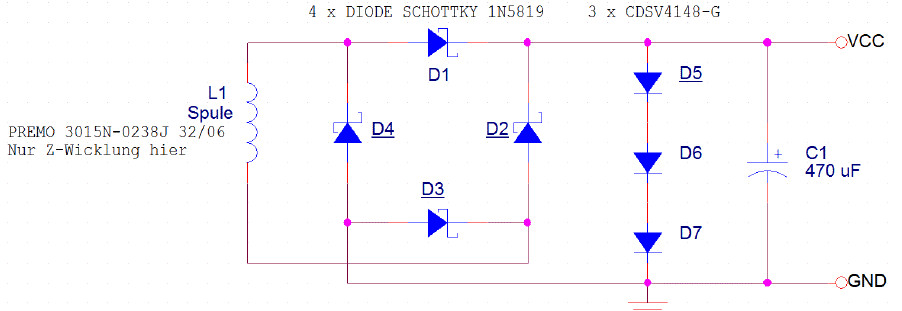
\includegraphics[width=0.5\textwidth]{3Vorgehen/imag/messschaltungHarvesterschaltung.jpg}
%    \caption{Messschaltung}
%\end{figure}
%
%\subsubsection*{Resultat}
%
%Die Rippelspannung erhöht sich wie erwartet. Vpp beträgt bei 100 uF \textbf{xx} mV, bei 47 uF 28.8 mV (siehe Abbildung \ref{kond47uF}) und bei 10 uF 320 mV (Abbildung \ref{kond10uF}).
% 
%\begin{figure}[ht]
%    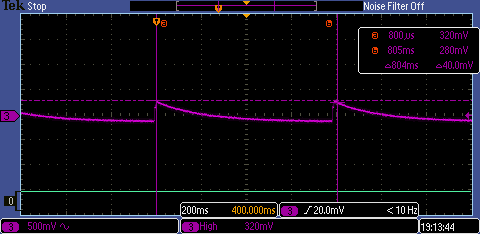
\includegraphics[width=0.5\textwidth]{3Vorgehen/imag/10uF.PNG}
%    \caption{Rippelspannung mit 10 uF Kondensator}\label{kond10uF} 
%\end{figure}
%
%\begin{figure}[ht]
%    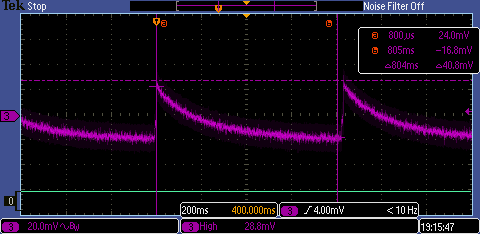
\includegraphics[width=0.5\textwidth]{3Vorgehen/imag/47uF.PNG}
%    \caption{Rippelspannung mit 47 uFKondensator}\label{kond47uF} 
%\end{figure}
%
%Nach Rücksprache mit einem Entwickler des EM8500-Chips wird der zu hohe Kondensator vor dem Harvester-Eingang als Ursache vermutet. Laut Datenblatt sollte dieser 4.7 $\mu$F, damit der Booster mit eingebautem MPPT ideal regeln kann.
%
Aus den Beobachtungen ergaben sich folgende Aufgaben für die Entwicklung des Prototypen:

\begin{enumerate}
    \item Die Harvesterschaltung funktioniert nicht optimal. Die Auswirkung des zu hohen Kondensator vor Harvestereingang soll getestet werden
    \item Die Schaltung soll für eine Geschwindigkeit von 10 km/h ausgelegt werden
    \item Die Konfigurationen beim EM8500 sollen überarbeitet werden, sodass LTS genutzt wird
    \item Das Senden der Pakte soll der Geschwindigkeit angepasst werden
\end{enumerate}

Punkte 1 und 2 haben Auswirkung auf das Layout, Punkte 3 und 4 auf die 





%------------------------------------------------------------------------------
% 2---------------------------------------------------------------------------
%------------------------------------------------------------------------------



\section{Hardware entwickeln}

Aus der Inbetriebnahme der Machbarkeitsstudie, wurden einige Punkte ersichtlich, welche mit einer neuen Leiterplatte, bzw. einer neuen Hardware verbessert werden können. Im speziellen muss die Harvesterschaltung genauer angeschaut werden und es soll versucht werden die nachfolgenden Punkte aus der Inbetriebnahme der Machbarkeitsstudie umzusetzen. 

\textit{Die Schaltung soll für eine Geschwindigkeit von 10 km/h ausgelegt werden.}

Ausserdem soll die neue Leiterplatte den fliegenden Aufbau der Harvesterschaltung und den EM-Chip beherbergen. Es wird in diesem Schritt darauf verzichtet, das TI-SensorTag ebenfalls in die neue Leiterplatte zu integrieren, da die Komplexität des TI-SensorTags hoch ist und die Hardware gut in mehreren Schritten überarbeitet werden kann.

\subsection{Schema}

Bevor ein Leiterplattenlayout entwickelt werden kann, muss das Schema erfasst werden. Es wurden verschiedenste Vorgaben von den Dozenten vorgegeben, welche im besten Fall alle eingehalten werden. Die Grösse der Leiterplatte soll die Grösse des TI-SensorTags nicht überschreiten, alle Netze sollen mit Testpunkten ausgestattet werden, alle Anschlüsse des TI-SensorTags auf der Leiterplatte zugänglich sein und alle Testpunkte des TI-SensorTags sollen im Rastermass 2.5 mm angeordnet werden. Ausserdem sollten, falls der Platz ausreichen würde, Strommesspunkte an der Speisung des TI-SensorTags, des Longterm Storage und des Shortterm-Storage angebracht werden. Diese Vorgaben sollen die Leiterplatte für eventuelle Laborübungen der Schule verwendbar machen. Das Schema besteht im groben aus vier Teilen:

\begin{enumerate}
    \item Harvesterschaltung
    \item EM-Chip inklusive zugehöriger Peripherie
    \item Energiespeicher
    \item Umlauferfassung
\end{enumerate}

\subsubsection{Harvesterschaltung}
Die Harvesterschaltung wurde in der Machbarkeitsstudie als fliegender Aufbau realisiert, was zu einigen Problemen führen kann, da viele lange Kabel verwendet wurden und somit die Signallaufwege ziemlich lang sind. Bisher hat dies keine Probleme verursacht, doch es geht wichtige Energie in den Kabeln verloren. Ebenfalls wurde in der Inbetriebnahme bemerkt, dass die gewonnene Leistung sehr gering ist, weswegen die Schaltung in einem zweiten Schritt optimiert werden muss.

\begin{figure}[ht]
    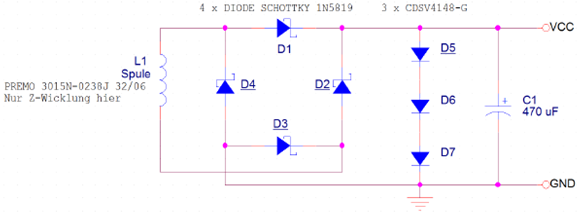
\includegraphics[width=0.5\textwidth]{3Vorgehen/imag/Schema_Harvester_PA.png}
    \caption{Harvesterschaltung der PA15}
    \label{schema_harvester_pa15} 
\end{figure}

Die Harvesterschaltung der Abbildung\ref{schema_harvester_pa15} wurde im Rahmen der Machbarkeitsstudie erarbeitet. Die Schaltung besteht aus wenigen Teilen, die Spannungbegrenzung wurde mit drei Dioden in Durchlassrichtung realisiert, hier gibt es wahrscheinlich bessere Möglichkeiten die Spannung zu begrenzen, ohne unnötig Leistung zu verschwenden.

\subsubsection{EM-Chip}

Das EM-Evaluationsboard soll ebenfalls auf der neuen Leiterplatte Platz finden, das Schema inklusive aller Kondensatoren ist im Datenblatt zu finden. Jedoch wurden die Jumper nicht übernommen und nur einige Stecker wurden übernommen, bzw. mit eigenen Signalen ergänzt.

\begin{figure}[ht]
    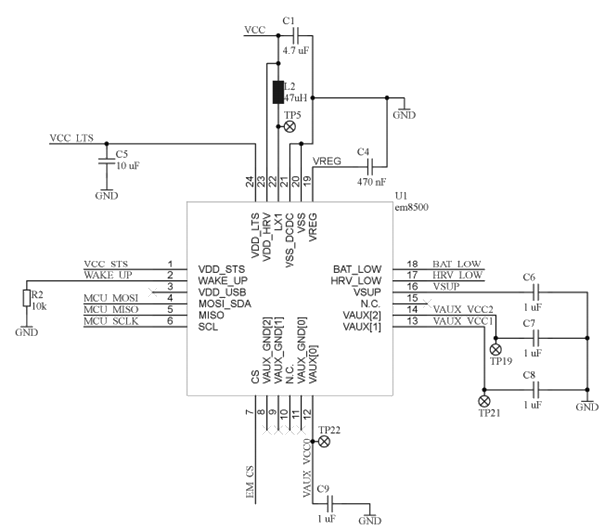
\includegraphics[width=0.5\textwidth]{3Vorgehen/imag/Schema_EM-Chip_inkl_Peripherie.png}
    \caption{Schema des EM-Chips mit der benötigten Peripherie}\label{schema_em-chip_inkl_peripherie} 
\end{figure}

\subsubsection{Energiespeicher}

Die Energiespeicher sollten flexibel gestaltet werden, da die genaue Art, bzw. Dimensionierung noch nicht definitiv war und noch Tests bezüglich der Energiespeicher anstanden. Jedoch wurde im Schema jeweils ein Elko als Platzhalter verwendet, da in der Machbarkeitsstudie ebenfalls Elkos verwendet wurden, die Kapazitätswerte sind jedoch nur erste Werte, welche nur abgeschätzt wurden.

\begin{figure}[ht]
    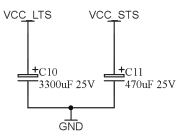
\includegraphics[width=0.5\textwidth]{3Vorgehen/imag/Schema_Energiespeicher.png}
    \caption{Schema der Energiespeicher (Elkos sind nur Platzhalter)}
    \label{schema_energiespeicher} 
\end{figure}

\subsubsection{Umlauferfassung}

Die Umlauferfassung kann nicht mit der verwendeten Spule realisiert werden, da die Energie aus der Spule gewonnen wird. Die nicht benutzten Wicklungen der X- und Y-Wicklung liefern kein klares Signal, was bereits in der Machbarkeitsstudie bewiesen wurde. Aus diesem Grund wird der Magnetdurchlauf mit einem Reedswitch detektiert und an das TI-SensorTag weitergegeben. Ein Magnetdurchlauf erzeugt einen positiven Puls, solange der Magnet in der Reichweite des Reedswitch befindet.

\begin{figure}[ht]
    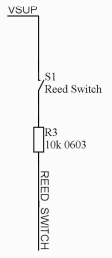
\includegraphics[width=0.1\textwidth]{3Vorgehen/imag/Schema_Umlaufdetektion.png}
    \caption{Schema Umlauferfassung}\label{schema_umlaufdetektion} 
\end{figure}

\newpage
\subsection{Bauteildefinition und Optimierung}

Nachdem klar war, welche Teile auf der Leiterplatte Platzfinden müssen, konnte die Optimierung der Schaltung in Angriff genommen werden. Ziel der Optimierung war es bei 10 km/h genügend Energie zu gewinnen, damit das TI-SensorTag damit versorgt werden könnte. Dafür musste vorallem die Harvesterschaltung optimiert werden, damit keine Energie unnötig verloren geht. 
Es wurden folgende Punkte angeschaut und versucht zu optimieren:

\begin{enumerate}
    \item die Spule
    \item der Gleichrichter
    \item der Limiter
\end{enumerate}

\subsubsection{Die Spule}

Die Spule gewinnt die Energie aus dem an einer Speiche des Fahrrads befestigten Magneten. Eine bessere Spule könnte mehr Energie aus dem vorbei schnellenden Magneten gewinnen. Entscheidend ist das die Fläche der Spule nicht vergrössert werden darf, bestenfalls sollte eine kleinere Spule gefunden werden, welche mehr Energie gewinnt. Gemäss der Formel 2.4 ist für die gewonnene Energie vor allem die Wicklungszahl entscheidend, jedoch wird bei den Spulen meistens nur die Induktivität angegeben. Dies ist kein Problem, da die Induktivität quadratisch von der Wicklungszahl (siehe Formel x) abhängt.

%\todo{Formel einfügen (Referenz: https://home.zhaw.ch/~spma/Scripts/ET_ST/EL2/Theorie/Induktivitaet.pdf (Konsultierung am 02.06.16))}

Es wurde nach einer Spule mit einer höheren Induktivität und der gleichen Fläche gesucht, somit können nur noch zwei Variablen sich verändern. Zum einen kann sich die Wicklungszahl verändern und zum andern kann sich die Länge der Spule verändern. Die Spule von Würth Elektronik hat eine ähnliche Fläche und eine grössere Induktivität, was auf den ersten Blick sehr vielversprechend aussieht.

Die Messung der erzeugten Spannung über der Spule hat ergeben, dass die Spule von Premo, welche bisher verwendet wurde, eine höhere Spannung erzeugt als die neue Spule von Würth. Die Spule von Premo mit der Bezeichnung 3015N 0238J 3206 hat bei den Geschwindigkeiten von 10 km/h und 20 km/h eine grössere induzierte Spannung. Die Spule von Würth mit der Bezeichnung 74458308 hat eine höhere Spannung bei den Geschwindigkeiten von 15 km/h und 40 km/h. Jedoch sollte die Schaltung für 10 km/h optimiert werden, somit muss der Spule von Premo der Vortritt gerwährt werden. Nachfolgend wird der Unterschied zwischen den induzierten Spannungen in den Spulen ersichtlich (siehe Abbildung \ref{messung_optimierung_spule}. Der Unterschied ist nicht gross, jedoch muss hier die Spule von Premo bevorzugt werden, da die induzierte Spannung grösser ist.

\begin{figure}[ht]
    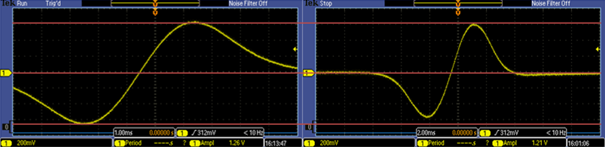
\includegraphics[width=0.5\textwidth]{3Vorgehen/imag/Messung_Optimierung_Spule.png}
    \caption{Links: Spannung über der Spule von Premo, Rechts: Spannung über der Spule von Würth, Geschwindigkeit 20 km/h}               
    \label{messung_optimierung_spule} 
\end{figure}

\subsubsection{Der Gleichrichter}

Der Gleichrichter aus der Machbarkeitsstudie bestand aus vier Dioden vom Typ 1N5819. Diese Dioden sind nicht für die LowPower-Anwendung ausgelegt, ausserdem sind die Dioden nicht ein einem Gehäuse verbaut. Wichtig ist bei dem Gleichrichter, dass die Leckströme möglichst klein sind und die Schwellenspannung sollte ebenfalls möglichst klein sein.

Es wurde als erstes eine LowPower-Diode, mit der Bezeichnung HSMS-286P, getestet, die Erwartungen waren entsprechend hoch, da diese Dioden für LowPower-Anwendungen spezialisiert ist. Die Spule von Premo wurde als Quelle verwendet, um zu sehen, wie die Spannung nach dem Gleichrichter aussieht. Die Spannung nach dem Gleichrichter bestehend aus den Dioden vom Typ 1N5819 ist bei allen getesteten Geschwindigkeiten, also 10 km/h, 15 km/h, 20 km/h und 40 km/h, höher als beim Gleichrichter bestehend aus den Dioden vom Typ HSMS-286P. Der Spannungsunterschied liegt im Minimum bei ca. 40mV. Der grösste Unterschied ist bei der Geschwindigkeit von 15 km/h ersichtlich, was in der Abbildung \ref{messung_optimierung_gleichrichter_1} gezeigt wird.

\begin{figure}[ht]
    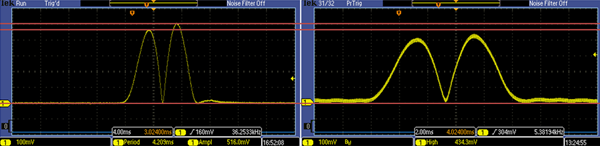
\includegraphics[width=0.5\textwidth]{3Vorgehen/imag/Messung_Optimierung_Gleichrichter_1.png}
    \caption{Links: Gleichrichter 1N5819, Rechts: Gleichrichter aus HSMS-286P, 15 km/h}
    \label{messung_optimierung_gleichrichter_1} 
\end{figure}

Als nächstes wurde ein Gleichrichter aus den Dioden vom Typ BAT54 getestet. Die Spannung nach dem Gleichrichter bestehend aus 1N5819 Dioden ist bei den Geschwindigkeiten von 15 km/h, 20 km/h und 40 km/h höher als nach dem Gleichrichter bestehend aus BAT54 Dioden. Der Spannungsunterschied liegt bei ca. 100 mVpp, der Unterschied ist marginal, jedoch muss hier der Gleichrichter aus 1N5819 Dioden bevorzugt werden. Nur bei einer Geschwindigkeit von 10 km/h ist der Gleichrichter bestehend aus BAT54 Dioden besser als der Gleichrichter bestehend aus 1N5919 Dioden. Der Spannungsunterschied liegt hier bei ca. 10mVpp, dieser Unterschied ist vernachlässigbar, in Angesicht, dass der Gleichrichter bestehend aus 1N5819 Dioden in allen anderen getesteten Geschwindigkeiten besser ist.

\begin{figure}[ht]
    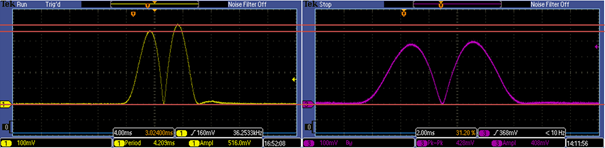
\includegraphics[width=0.5\textwidth]{3Vorgehen/imag/Messung_Optimierung_Gleichrichter_2.png}
    \caption{Links: Gleichrichter 1N5819, Rechts: Gleichrichter aus BAT54, 15 km/h}
    \label{messung_optimierung_gleichrichter_2} 
\end{figure}

\subsubsection{Der Limiter}

Die Spannungsbegrenzung, nachfolgend der Limiter genannt, ist ein sehr krititscher Teil der Harvesterschaltung, da die Spannung am EM-Chip Eingang nicht höher als 2 V sein darf, da ansonsten der EM-Chip beschädigt werden kann. Trotzdem soll möglichst wenig Energie verloren gehen, wenn die Spannungsbegrenzungsschaltung ihre Arbeit verrichtet. Bisher wurden drei Dioden in Durchlassrichtung in Serie geschalten, um die Spannung zu begrenzen.

Herr Erich Ruff hat eine Spannungsbegrenzungsschaltung entwickelt, welche er uns freundlicherweise zur Verfügung stellte. Diese Schaltung wurde mit dem Limiter verglichen, welcher aus drei Dioden bestand.

Die Spannung nach dem Dioden-Limiter ist bei 10 km/h, 15 km/h und 20 km/h höher, jedoch ist die Rippelspannung ebenfalls höher. Nur bei einer Geschwindigkeit von 40 km/h ist die Spannung nach dem LImiter von Herr Erich Ruff, nachfolgend FET-Limiter genannt, besser sowohl bei Spannungslevel als auch bei der Rippelspannung. Die Abbildung x zeigt, dass der Dioden-Limiter eine höhere Spannung liefert, jedoch ist die Rippelspannung ebenfalls höher.

\begin{figure}[ht]
    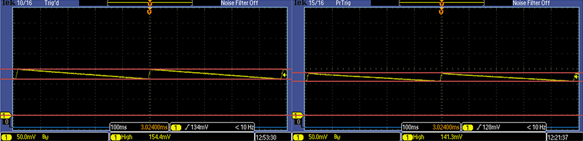
\includegraphics[width=0.5\textwidth]{3Vorgehen/imag/Messung_Optimierung_Limiter.png}
    \caption{Links: Dioden-Limiter, Rechts: FET-Limiter, 15 km/h}\label{messung_optimierung_limiter} 
\end{figure}

\subsection{Layout}

Schlussendlich musste aus den optimierten Teilen des Schemas eine Leiterplatte gestaltet werden. Die meisten Footprints waren bereits in den Bibliotheken des IneS vorhanden, einige mussten neu gezeichnet werden.

\subsubsection{Positionierung}

Die Positionierung der einzelnen Teile kann sehr wichtig sein, da mit einer guten Positionierung bereits unnötige Leiterbahnverläufe verhindert werden können. Ebenfalls können gut positionierte Bauteile die Spannungspegel stabilisieren. Es wurde darauf geachtet die Bauteile, welche zu einem Block gehören, nahe beieinander platziert wurden, um unnötig lange Signallaufwege zu verhindern.

Die Bauteile der Harvesterschaltung wurde als Block so nahe wie möglich beieinander platziert und wo immer möglich wurden die Speisungsleitungen mit 20 Mil gezogen, damit der Widerstand der Leiterbahn möglichst klein gehalten wurde. Der Leiterwiderstand konnte so minimiert werden, was verhindert, dass die Energie in den Leiterbahnen verschwendet wird.

\todo{Formel für Leiterwiderstand einfügen}

Der Widerstand bei 10 Mil ist somit 2.4 m$\Omega$, 
der Leiterwiderstand bei einer Leiterbahnbreite von 20 Mil ist 1.2 m$\Omega$. 
Problematisch ist, dass der Block der Harvesterschaltung etwas entfernt vom Block des EM-Chips befindet, das bedeutet, die Leiterbahn mit der Speisung des EM-Chips muss mehrere Zentimeter zurücklegen. Sicherlich ist der Unterschied im Widerstand nicht sehr gross, doch die Energie, welche in der Leiterbahn verloren gehen würde, konnte so halbiert werden.

Der wichtigste Aspekt der Platzierung des EM-Chips war, dass die Stützkondensatoren so nah wie möglich am EM-Chip platziert wurden, damit die Spannung am EM-Chip so konstant wie irgend möglich gehalten werden kann.

Ein weiterer wichtiger Punkt war die Platzierung des Steckers, welcher unsere Leiterplatte mit dem TI-SensorTag verbindet, durch eine Falschplatzierung kann es hier passieren, dass die beiden Leiterplatten nicht schön übereinander sind, wenn sie aufeinander gesteckt werden. Das ist eher ein ästhetisches Problem, jedoch kann das auch Problem beim Einbauen in ein eventuelles Gehäuse bereiten. Zu dem Stecker gehört auch die Paltzierung der Testpunkte, welche direkt mit dem Stecker verbunden sind. Gemäss dem Wunsch der Betreuer wurde hier ein Rastermass von 2.5mm der Testpunkte eingehalten, so dass eine Steckerleiste eingelötet werden könnte. Problematisch ist jedoch, dass die Testpunkte einen grossen Raum der Leiterplatte einnehmen, wie in Abbildung \ref{layout_testpunkteraster} ersichtlich.

\begin{figure}[ht]
    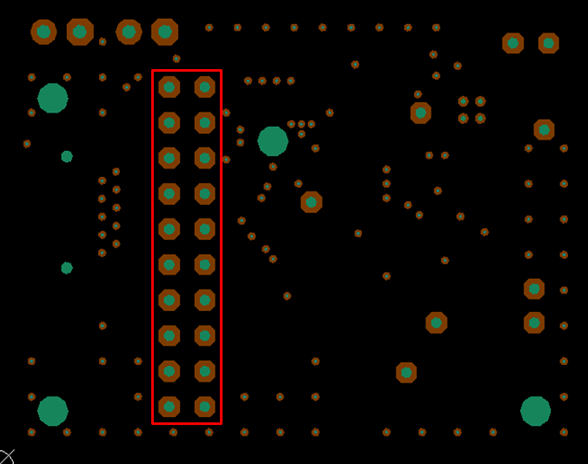
\includegraphics[width=0.5\textwidth]{3Vorgehen/imag/Layout_Testpunkteraster.png}
    \caption{Pads der Leiterplatte, rot eingerahmt die Testpunkte des Steckers}\label{layout_testpunkteraster} 
\end{figure}

\subsubsection{Das erste Layout}

Die erste Version der Leiterplatte war mit vielen Wünschen der Betreuer ausgestattet. Alle Netze wurden mit Testpunkten ausgestattet, die Testpunkte des Steckers wurden im Rastermass 2.5mm angeordnet und die Netze der Spannung nach dem Harvester, die Spannung des Short- und Long-Term-Storage wurden mit Strommesspunkten ausgestattet. Es wurden ebenfalls Montagelöcher platziert, jedoch sind diese sehr minimalistisch, da nur eine M2-Schraube durch passt, besser wäre es Montagelöcher für M3-Schrauben zu platzieren, doch der Platz auf der Leiterplatte ist sehr limitiert. Die Leiterplatte ist nur 33x42mm gross, was ein Milimeter breiter ist, als das TI-SensorTag. Der Anschluss der Energiespeicher wurde so realisiert, dass die Energiespeicher nicht auf der Leiterplatte Platz finden, sondern über ein Kabel oder Litze mit der Leiterplatte verbunden werden können.

\subsubsection{Das Redesign}

Ein grosser Fehler wurde in der Umsetzung des Steckers begangen, denn sowohl die Platzierung als auch der Footprint wurden falsch umgesetzt. Der Stecker wurde nicht an der richtigen Stelle platziert, somit überlappte unsere Leiterplatte das TI-SensorTag. Beim Erstellen des Footprints des Steckers wurden die Pins vertauscht, dort wo der Pin 1 sein sollte wurde der Pin 19 platziert und umgekehrt. Dies musste korrigiert werden, damit unsere Leiterplatte direkt mit dem TI-SensorTag verbunden werden kann. Dafür wurde die Leiterplatte überarbeitet, jedoch war die Zeit zu knapp, als dass die Leiterplatte für Tests vorhanden war.

\begin{figure}[ht]
    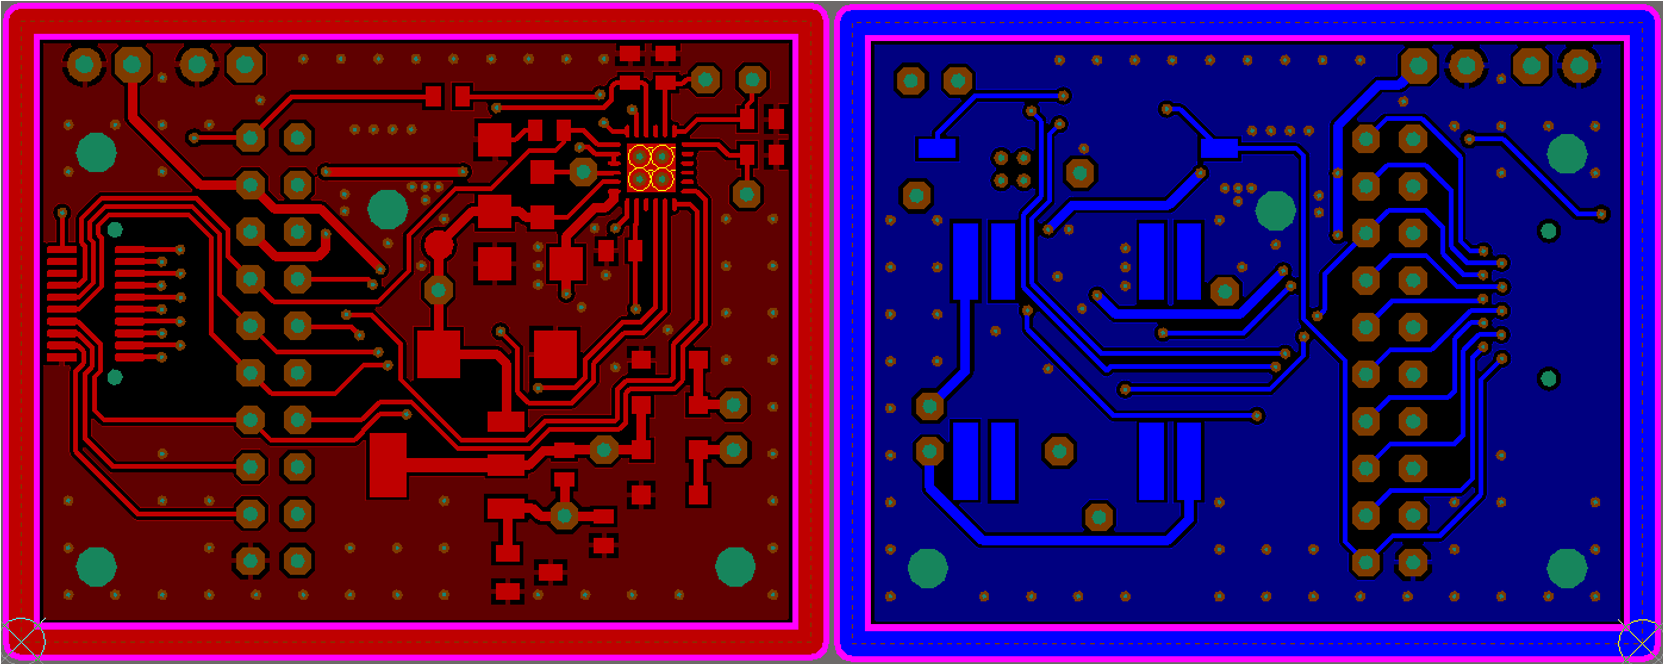
\includegraphics[width=0.5\textwidth]{3Vorgehen/imag/Layout_Redesign.png}
    \caption{Links: Top-Layer, Rechts: Bottom-Layer}\label{layout_redesign} 
\end{figure}

\todo{ Namensklärung: V HRV = VCC}
\todo{Messprotokolle umbenennen}

% 4----------------------------------------------------------
\section{Inbetriebnahme des Prototypen}
Ziel des Kapitels: Ausmessen und sehen, dass zu wenig Energie. (Weglassen. Testteil). 2. Magnete nach 180 \% (Bild), Reellight bringt idee für 2 Magnete hintereinander, besser Spule verwenden

--- alter Text
Der entwickelte Prototyp wurde intensiv ausgemessen (siehe Messprotokolle XXXX.)  Es werden 3 Messstellen unterschieden siehe Abbildung \ref{EnergieMessungStellen}. In den folgenden Unterkapiteln werden die Resultate und die darauf folgenden Entwicklungsschritte kurz beschrieben:

\begin{figure}[ht]
  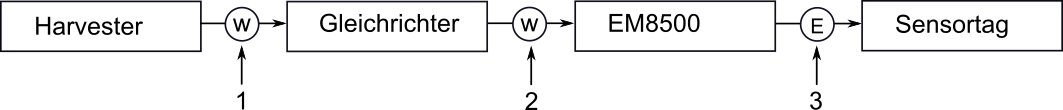
\includegraphics[width=1.0\textwidth]{3Vorgehen/imag/EnergiemessungStellen.png}\label{EnergieMessungStellen} 
  \caption{Messstellen am Prototypen}
\end{figure}

\subsection{Testen der Harvesterschaltung}

- Zu wenig Energie
- Zwei Magnete
- stärkere Spule

\subsection{Ausmessen der Energie vor und nach dem Gleichrichter}


\subsection{Energiemessungen nach dem EMBoard}



% 5---------------------------------------------------------------------------
\section{Energy Management}

Das Ziel des Energy Managements ist es, dass die zur Verfügung stehende Energie bei 10 km/h genügt, um BLE-Pakete zu versenden. Die sekundäre Aufgabe ist es, dass sich der Long Time Storage lädt und entlädt. Ein Laden des LTS ohne Energieabgabe ist Energieverschwendung. Die zwei gestellten Aufgaben sollen durch möglichst optimale Speichergrössen und intelligente Schwellwerte erreicht werden.

Damit man die Kondensatorenwerte berechnen kann, braucht es Energiedaten. Deshalb stehen als erstes im Unterkapitel \ref{v_messungen_sensortag} die Energie-Messergebnisse, danach folgt im zweiten Unterkapitel \ref{v_e_kalkulation} die Dimensionierung der Kondensatoren und dann das Berechnen der Schwellwerte in Unterkapitel \ref{v_schwellwerte}. Als letzer Punkt werden die Energiezustände innerhalb des Bicycle Computers definiert. Dies, weil die letzte offene Aufgabe der Optimierunsliste (\ref{optimierung}) das Senden nach 10 s dem Energiezustand angepasst werden soll.


% x.1 ------------------------
\subsection{Energiemessungen}
\label{v_messungen_sensortag}


Die Entwicklung ist konstant begleitet durch Energiemessungen. Sei dies durch Leistungsmessungen bei der Hardware (Harvester und EM8500-Chip) oder sei dies als Energiemessung der Software (TI-SensorTag). Für die Energiemessungen wird der Power Analyser von Agilent Electronic N6705B mit der Serienummer MY50000795 gebraucht. Dieses mächtige Messgerät misst gleichzeitig Strom, Spannung und Leistung im Zeitverlauf. Mühsame Annäherungen aus en KO-Messungen sind nicht mehr notwendig.

In diesem Unterkapitel werden die Resultate den TI-SensorTag-Energiemessungen. Mehr Messgraphiken und Erklärungen sind in der Datei \todo{referenz} abgelegt. Den Überblick über die Versionen ist in der untenstehenden Tabelle aufgelistet. 


\subsubsection{Überblick Energiemessungen}
\label{erst_EMessungen}

\begin{figure}[ht]
    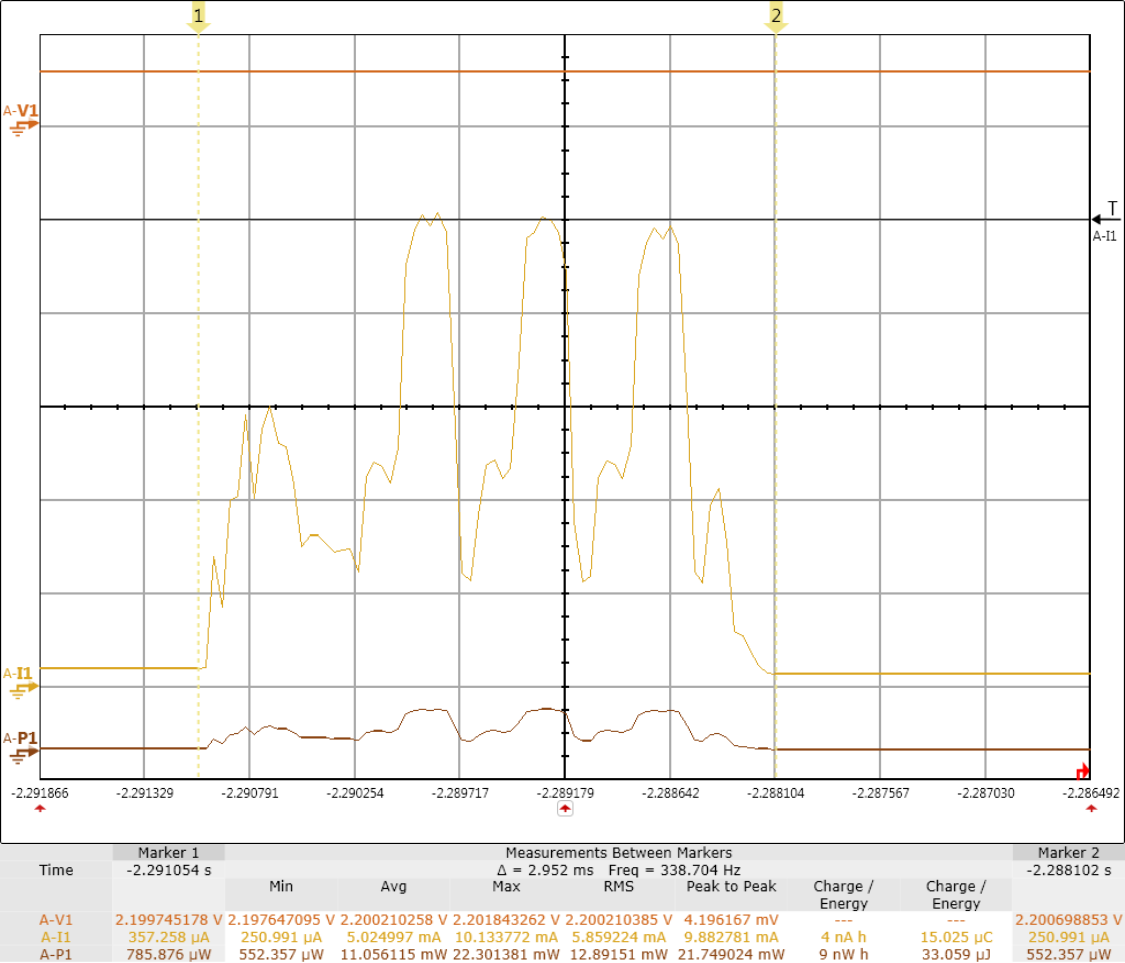
\includegraphics[width=0.5\textwidth]{3Vorgehen/imag/v0Send33uJ.png} 
    \caption{Minimalster Energieverbrauch: 3 BLE Pakte über Advertising Mode senden}
    \label{BLE_send}
\end{figure}

Um einen ersten Anhaltspunkt über den Energieverbrauch des TI-SensorTags zu erhalten, werden drei BLE-Pakete im Advertsing Mode per Knopfdruck gesendet (siehe Abbildung \ref{BLE_send}). Dies entspricht der Messung zur TI-SensorTagversion V0. Nach der Weiterentwicklung des Programms zum Auslesen der Sensoren, folgte die Messung V1. In dieser Version wird die GPIO ausgelesen. Die GPIO ist für das Einlesen der Reed Switch-Impulse unumgänglich. Die Version V2, der Versuch mehr Sleep-Time einzubauen, scheiteret am Zusammenspiel des Timings der BLE-Radio-Interrupts mit den GPIO-Interrupts. Durch das Neuaufsetzen des Programms entsteht die Version V3. Diese sendet power-optimiert Geschwindigkeitspakete. 

Die untenstehende Tabell stellt dieEnergieresultate dar. Unterschieden wird zwischen dem Energieverbrauch für die Initialisierung, kurz Init, und der Energie zum Senden von drei BLE-Paketen. Die Diskussion über Energieoptimierungen und die Deutung der Resultate finden sich in den Sitzungsprotokollen vom xxxxx - xxxx. 

\todo{Sitzungsprotokolle Datum einsezten, Anhanhgsbezeichnung}

\subsubsection*{Messresultate nach TI-SensorTag-Versionen}
\begin{tabbing}
    Version   \quad\= Datum    \quad\= Was................................................... \quad\= Energie Init    \quad\=  Energie Senden \\[0.8ex]
    V0        \> 10.3.16  \> Nur BLE Paket      \> unbekannt            \> 33 $\mu$J \\
    V1        \> 16.3.16  \> mit Geschwindigkeit      \> 87 $\mu$J            \> 32 $\mu$J \\
    V3        \> 22.4.16   \> Schlafmodus optimiert     \> 40 $\mu$J            \> 29 $\mu$J \\
    V4        \> 03.6.16    \> 3 Sensore, kein Schlafmodus optimiert     \> 77 $\mu$J            \> 43 $\mu$J \\
    V5        \> ongoing    \> 3 Sensore mit optimiertem Schlafmodus     \> 77 $\mu$J            \> 43 $\mu$J \\
\end{tabbing}

Bei den ersten drei Messungen werden die Sensoren noch nicht ausgelesen. Es zeigt sich, dass das Auslesen der Sensoren über I2C und das Warten, bis dass die Sensoren gestartet sind,  mehr Energie verbraucht, als erwartet. Der Energieverbrauch für das Auslesens eines Sensors ist ohne Optimierungsmassnahmen so gross, dass kein Senden der Daten möglich ist. Die Speisung der Applikation bricht zusammen (siehe Abbildung \ref{i2c_problem}).

\begin{figure}[ht]
    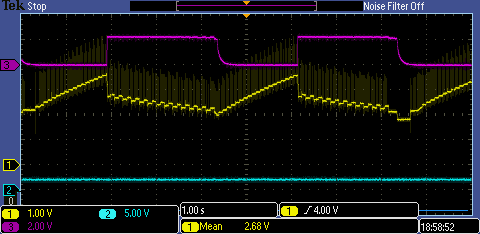
\includegraphics[width=0.5\textwidth]{3Vorgehen/imag/pic4VSUPbrichtEin.PNG} 
    \caption{Auslesen der Sensoren reisst Energie zusammen}
    \label{i2c_problem}
\end{figure}



Aus diesen Grund wurde die Poweroptimierung innerhalb des Programms zur zentralen Herausforderung in dieser Arbeit. Details darüber sind im nächsten Unterkapitel (\ref{powerOptimierung} Power Management) zusammengefasst. Bei der Version V4 zeigt sich, dass die Funktion BLE-Send, zu der auch das Einlesen der Sensordaten gehört, ein Zuwachs von 50 \% an Energiebedarf bewirkt. 



\subsubsection{Resultate Energieverbrauch TI-SensorTag Applikation V4}
\label{energie senosortag} 

Als Überblick über den konkreten Energieverbrauch bei der Version V4 folgt exemplarisch ein Bild zur Initialisierung (Abbildung \ref{energie_init}), eines zum Senden der drei BLE-Pakete (Abbildung \ref{energie_senden})und dann je eine Abbildung zum Energieverbrauch beim Starten der drei Sensoren.

\begin{figure}[ht]
  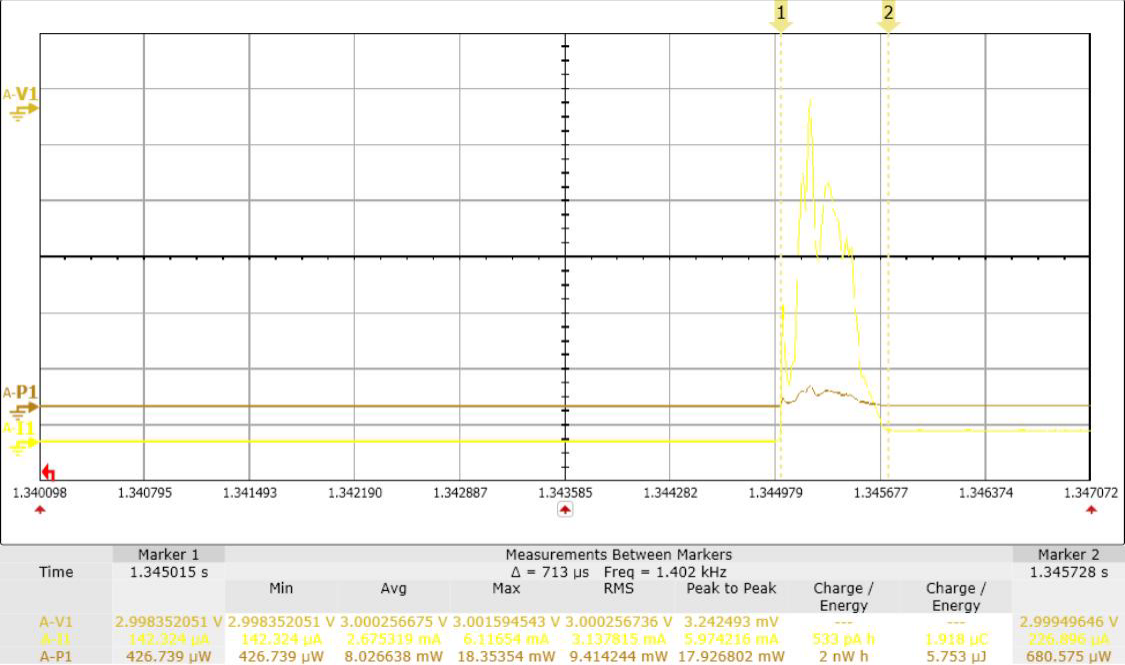
\includegraphics[width=1.0\textwidth]{3Vorgehen/imag/Drucksensor.png}
  \caption{Energieverbrauch für Initialisierung}
  \label{energie_init}
\end{figure}

\begin{figure}[ht]
  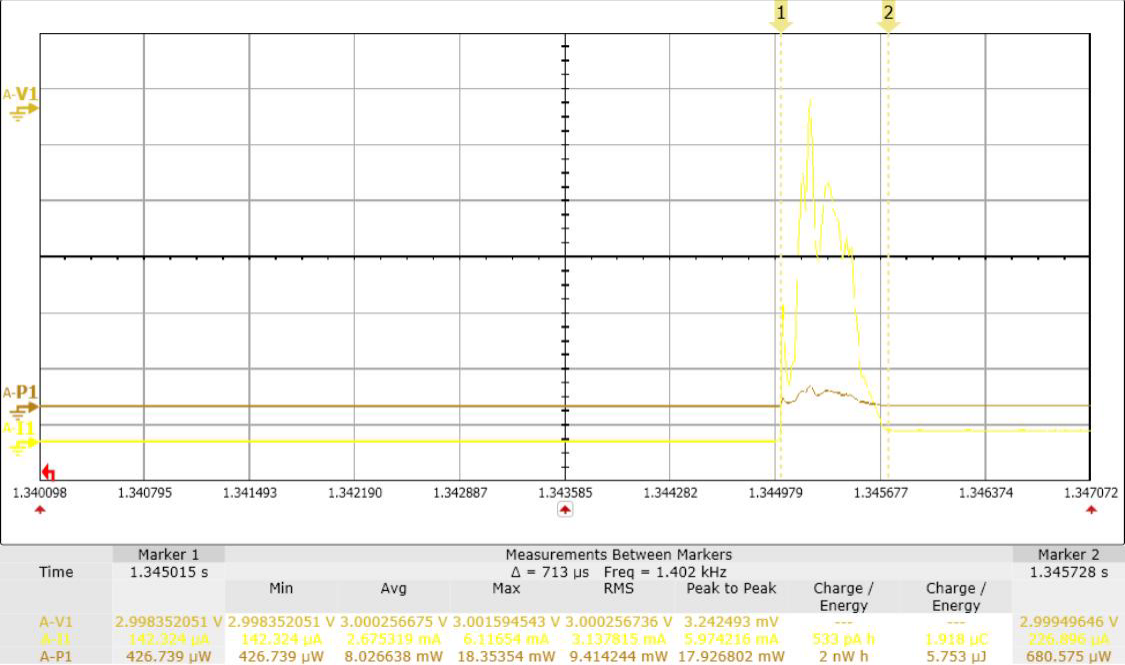
\includegraphics[width=1.0\textwidth]{3Vorgehen/imag/Drucksensor.png}
  \caption{Energieverbrauch senden eines BLE-Paketes mit Sensordaten}
  \label{energie_senden}
\end{figure}


\paragraph{Energieverbrauch Starten des Drucksensors}

Auf dem TI-SensorTag wird der Drucksensor BMP 208 von Bosch Sensortec verwendet. Weil der Drucksensor lange \todo{Zeit einfügen} braucht, um zu starten, wird dieser Vorgang in eine eigene Funktion ausgelagert. Hier die Energiemessung des Startvorgangs des Sensors, ausgelesen mit der TI-SensorTag Version 4, am 3. Juni 2016. Die Version V4 ist noch nicht vollständig power-optimiert.

\begin{figure}[ht]
  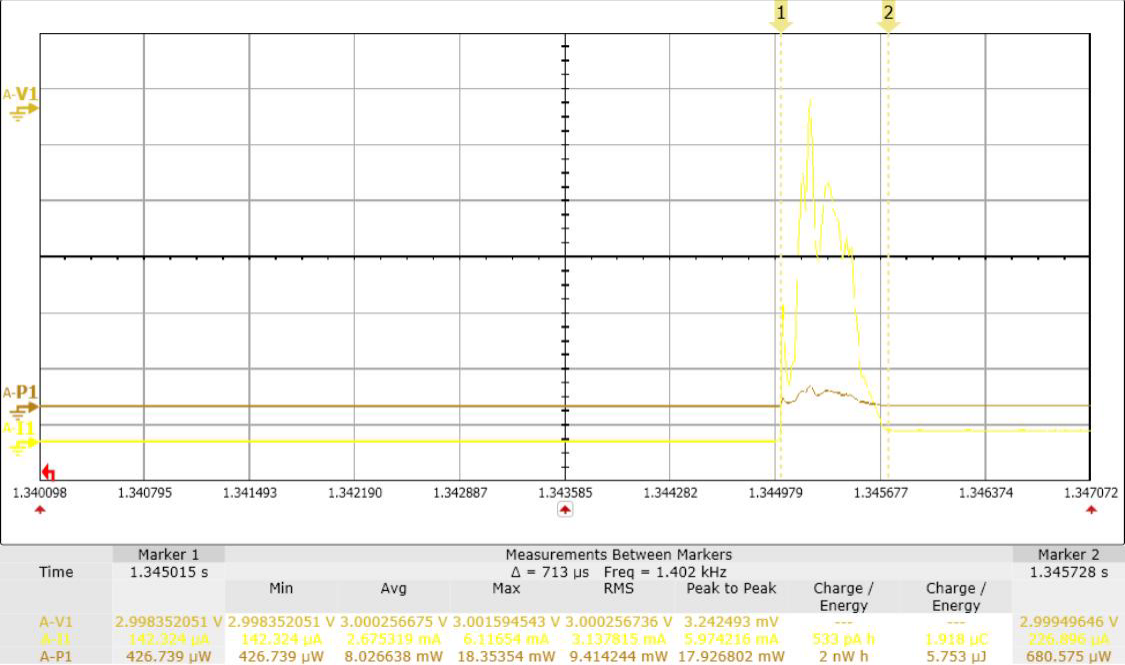
\includegraphics[width=1.0\textwidth]{3Vorgehen/imag/Drucksensor.png}
  \caption{Energieverbrauch des Drucksensors BMP 280}
  \label{energie_drucksensor}
\end{figure}

Das Starten des Drucksensors verbraucht 5.753 $\mu$J.

\paragraph{Energieverbrauch beim Starten des Temperatursensor}

\todo{tempsensor daten}
Der Temperatursensor xxx der Marke yyy verbraucht fürs Auslesen der Daten, ohne Energieoptimierung, 10.635 $\mu$J.

\begin{figure}[ht]
  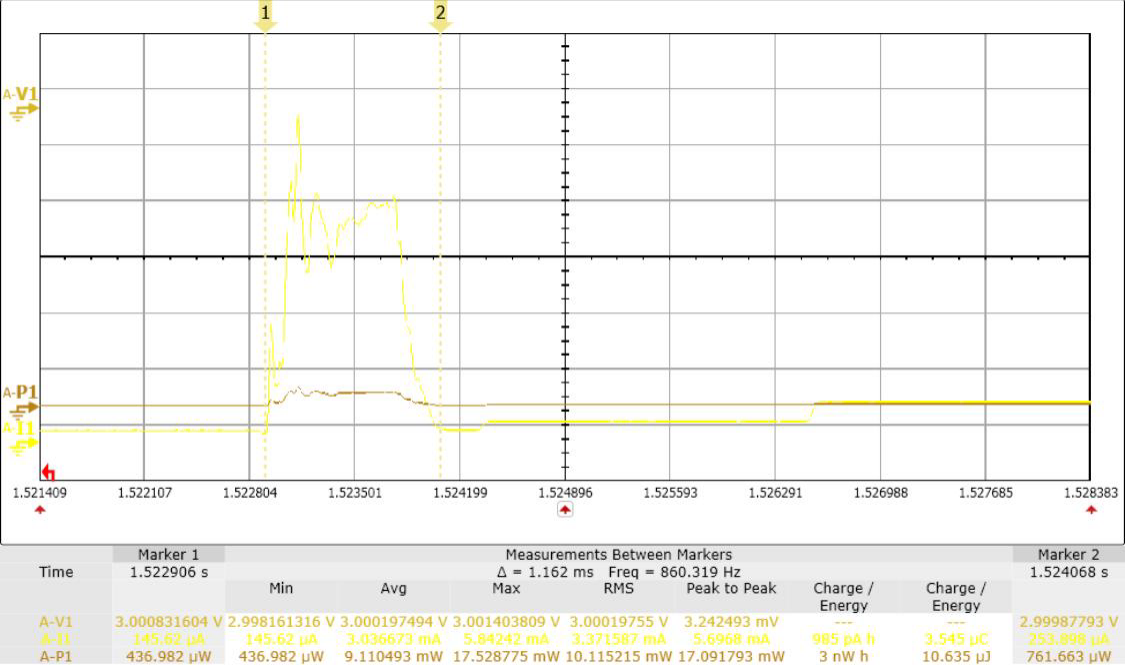
\includegraphics[width=1.0\textwidth]{3Vorgehen/imag/tempSensor.png}
  \caption{Energiemessung Temperatursensor auf TI-SensorTag}
  \label{energie_tempsensor}
\end{figure}


\paragraph{Energieverbrauch Feuchtigkeitssensor}

Der Feuchtigkeitssensor verbraucht 6.358 $\mu$J, siehe Abbildung \ref{energie_humidity}.

\begin{figure}
  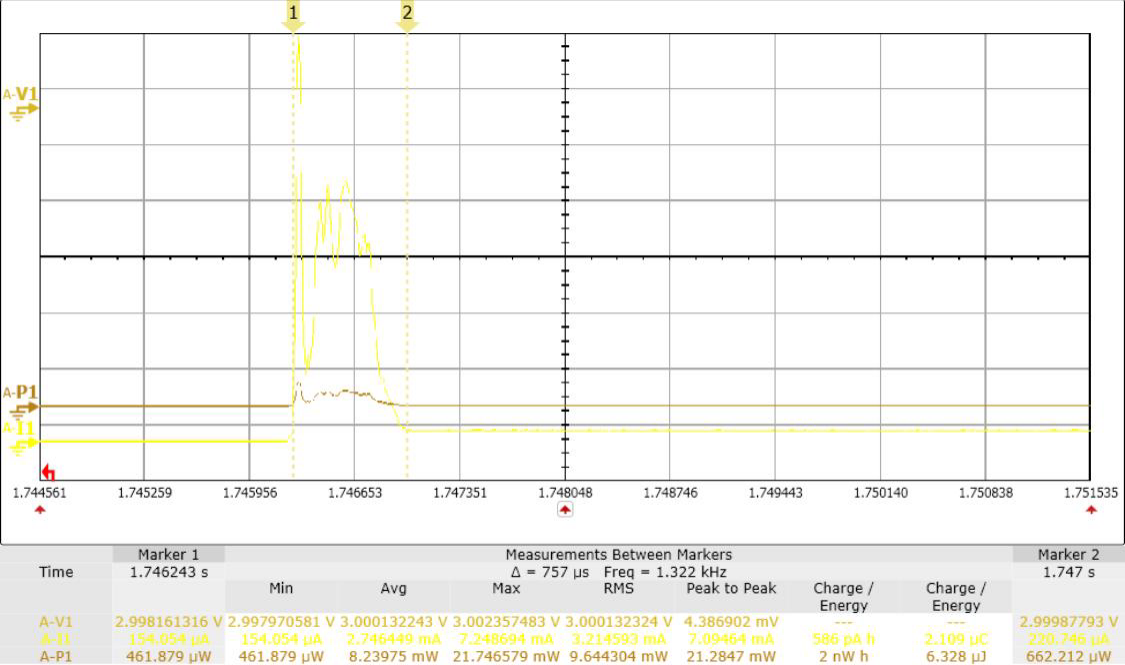
\includegraphics[width=1.0\textwidth]{3Vorgehen/imag/Humidity.png}
  \caption{Energieverbrauch Feuchtigkeitssensor}
  \label{energie_humidity}
\end{figure}




% x.2 ---------------------------------
\subsection{Energiekalkulation}
\label{v_e_kalkulation}

Der Energieverbrauch hängt von der Anzahl ausgelesener Sensoren ab (siehe \ref{v_messungen_sensortag}). Für die Bestückung der Kondensatoren wird vom schlechtesten  Fall, einer Geschwindigkeit von 10 km/h ausgegangen. Die Grundlagen zur Energiekalkulation $\bar{E_{HRV}} \ge \bar{E_{BLE}} $ sind im Theorieteil \ref{th_energiebilanz} abgebildet. Hier werden die Kondensatoren berechnet.

\todo{Gleichungen zusammen. Berechnung konkret}
\begin{equation}
  C_{STS}= \frac{ E_{Applikation}}{(V_{STS\_HIGH} )^2 - (V_{STS\_LOW} )^2}
\end{equation}

\begin{equation}
  C_{STS}= \frac{ E_{Applikation}}{(3.6 V )^2 - (2.1 V)^2}
\end{equation}

\begin{equation}
  C_{STS}= \frac{ E_{Applikation}}{(3.6 V )^2 - (2.1 V)^2}
\end{equation}

\begin{equation}
  C_{STS}= \frac{ E_{Applikation}}{(3.6 V )^2 - (2.1 V)^2}
\end{equation}


\todo{Abschlusstext. Übergang}

\subsubsection{MPP einstellen}

\todo{Messprotokolle eintrage}

Das Ziel der Entwicklung ist, dass bei einer Geschwindigkeit von 10 km/h genug Enerige zum Senden eines BLE-Pakets zur Verfügung steht. Während der Entwicklung des Harvesters wurde die Leistungskurve öfters aufgenommen (siehe Anhang \ref{uebersicht_messprotokolle}, xxx,yyy, zz). Wie im Theorieteil erklärt \ref{harv_diff} unterscheidet sich das Leistungsmaximum nach Geschwindigkeit. Weil das Ziel ein funktionstüchtiger Prototyp bei 10 km/h ist, bezieht sich das Einstellen nur auf diese Wert.  

 
\subsubsection*{MPP-Ratio bei 10 km/h gemäss Messprotokollen}
\begin{tabbing}
    Datum       \quad\= Leistungmaximum    \quad\= MPP-Ratio\\[0.8ex]
    30. März    \> 12 $\mu$W        \> 43.23\thinspace\% \\
    xx          \> xx $\mu$W        \> xx\thinspace\%\\
    resultat    \> 21.87  $\mu$W    \> 24.87\thinspace\%\\
\end{tabbing}\todo{Werte}

Es zeigt sich, dass das Leistungsmaximum unterhalb von 50\thinspace\% liegt. Bedauerlich ist, dass durch die Energieoptimierung sich die Stelle des Leistungsmaximums Richtung Leerlauf verschiebt. In der Umsetzung mit dem EM8500-Chip ergibt sich das Problem, dass nur Konfigurationen von MPPT-Ratios von 50 - 80\thinspace\% erlaubt sind (siehe Tabelle unten).  Die Einstellungen der tieferen MPP-Ratio sind zudem gröber. Dies, weil der EM8500-Chip für Harvester vom Typ TEG (mit einem MPP konstant bei 50\thinspace\%) und Solarzelle konzipiert ist und die MPPT-Ratio für diese zwei Anwendungen genau in diesem Range liegen. In unserem Fall ist dieser vorgegebene Range nicht ideal. Da beim energiekritischen Zustand bei 10 km/h die Ratio deutlich unter 50\thinspace\%. Die Vorgänger wählten in ihren Einstellungen eine MPPT-Ratio von 88\thinspace\%. Die Vermutung liegt nahe, dass keine Leistungskurve des Harvesters im Voraus aufgenommen wurde.


\subsubsection*{MPPT-Ratio Einstellungen EM8500}
\begin{tabbing}
    Registerwert   \quad\= MPPT-Ratio    \\[0.8ex]
    0x00           \> 50\thinspace\% \\
    0x01           \> 60\thinspace\%\\
    0x02           \> 67\thinspace\%\\
    0x03           \> 71\thinspace\%\\
    0x04           \> 75\thinspace\%\\
    0x05           \> 78\thinspace\%\\
    0x06           \> 80\thinspace\% \\
    0x07           \> 82\thinspace\%\\
    0x08           \> 83\thinspace\%\\
    0x09           \> 85\thinspace\%\\
    0x0A           \> 86\thinspace\% \\
    0x0B           \> 87\thinspace\%\\
    0x0C           \> 88\thinspace\%\\
\end{tabbing}

\todo{Sitzungsprotokoll Datum}
Im ersten Versucht wird das Register auf das Minimum (50\thinspace\%) eingestellt (siehe Sitzungsprotokoll YYYY). Die Messung ergab, dass bei 10 km/h das EM-Board nicht gespiesen wird. So luden sich weder der STS noch der LTS auf. Der Grund ist, dass der optimale Leistungsbezug bei 50\thinspace\% liegt, das Leistungsmaximum aber später. So entstand beim Regeln auf den optimalen Leistungsbezug der Umstand, dass dort nur 0.2 V produziert werden. Dieser Spannungswert ist zu tief, der EM-Chip beginnt nicht zu arbeiten. Betreibt man den Harvester nicht am optimalen Punkt, sondern bei einer MPPT-Ratio von 60\thinspace\%, so wird eine Eingangsspannung von 0.3 V produziert und EM8500 beginnt zu arbeiten.




% x.3 -------------------------------------
\subsection{Einstellen der Schwellwerte}
\label{v_schwellwerte}

Das Konzept der Schwellwerte von VSTS und VLTS sind im Theorieteil bei der Erklärung des Speicherkonzepts des EM8500-Chips im Unterkapitel \ref{speicher_konzept} beschrieben. Das Ziel ist, dass bei 10 km/h sich LTS entlädt. Die Berechnung der Schwellwerte stammt aus dem Theorieteil \ref{th_energiebilanz}.




Aus der Vorgängerarbeit sind in der Tabelle unten notierte Konfigurationswerte überliefert. Bei der Inbetriebnahme fiel der hohe Schwellwert von v\_bat\_min\_hi\_dis auf (3.6 V), ab der erst die Applikation gespiesen wird. Den hohen Wert beruht auf dem Versuch, möglichst viel Energie vor dem Datensenden zu sammeln. Ein hoher Schnellwert verzögert die Zeit, bis zum ersten Datensenden.

\subsubsection*{Konfiguration Vorgängermodell}
\begin{tabbing}
    Register .............\quad\= Wert \\[0.8ex]
    v\_bat\_max\_hi       \> 4.2 V \\
    v\_bat\_max\_lo       \> 4.1 V \\
    v\_bat\_min\_hi\_dis  \> 3.6 V \\
    v\_bat\_min\_hi\_con  \> 2.1 V \\
    v\_bat\_min\_lo       \> 1.8 V \\
    v\_appl\_max\_hi      \> 3.8 V \\\
    v\_appl\_max\_lo      \> 3.7 V \\ 
    mppt\_ratio            \> 88\thinspace\% \\
\end{tabbing}

Nach der Energiemessungen der Version V3 des TI-SensorTags (siehe \ref{erst_EMessungen}), in dem die Geschwindigkeit per BLE gesendet werden kann, entstanden folgende Schwellwerte:

\subsubsection*{Erste Konfiguration aufgrund Geschwindigkeitsmessung}
\begin{tabbing}
    Register .............\quad\= Wert \\[0.8ex]
    v\_bat\_max\_hi       \> 4.8 V \\
    v\_bat\_max\_lo       \> 4.7 V \\
    v\_bat\_min\_hi\_dis  \> 2.6 V (siehe Berechnungen unten)\\
    v\_bat\_min\_hi\_con  \> 2.1 V \\
    v\_bat\_min\_lo       \> 2.0 V (vorgegeben von TI-SensorTag)\\
    v\_appl\_max\_hi      \> 3.8 V \\\
    v\_appl\_max\_lo      \> 3.7 V \\ 
    mppt\_ratio            \> 50\thinspace\% (aus MPP-Kurve Harvester)\\
\end{tabbing}

Die Grundlage bildete die Gleichung  $E_{Applikation}= E_{STS\_HIGH} - E_{STS\_LOW}$, wobei  $E_{Applikation}$ aus der Messung von V3 mit total 93.2 $\mu$J für die Initialisierung und das Senden der Daten gebraucht werden, und $V_SUP$ durch das TI-SensorTag mit 2.0 vorgegeben ist. Laut Datenblatt des EM8500 (\cite{datasheet_EM85}, S. 9, Abschnitt Operating Conditions ) soll STS zwischen 10 - 100 $\mu$F gross sein. Typisch ist 47 $\mu$F. Um auf der sicheren Seite zu sein, denn der Harvester gibt zu diesem Zeitpunkt noch nicht genug Energie ab, wurde als Berechnungsgrundlage C\_{STS} von 100 $\mu$F genommen.  So ergab sich folgender minimaler oberere Schwellwert:

\begin{equation}
(v\_bat\_min\_low) ^2  =  \frac{2\, \times \, E_{Applikation}}{C_{STS}} + (V_{STS\_LOW})^2
\end{equation}

\begin{equation}
(v\_bat\_min\_low) ^2  =  \frac{2\, \times \, 93.2, \mu J}{100 \,\mu F} + (2.0)^2
\end{equation}

\begin{equation}
v\_bat\_min\_low  =  \sqrt{\frac{186.4}{100 } + 4} = \sqrt{5.864} = 2.42 V
\end{equation}

Alternativ kann man den laut Datenblatt vorgeschlagenen Kondensatorenwert von  47 $\mu$F. Dann ergibt sich als oberer Schwellwert  $v\_bat\_min\_low  =  \sqrt{\frac{186.4}{47 } + 4} = \sqrt{7.97} = 2.82, V$. Als erstes wird der Schwellwert auf 2.6 V gesetzt. Wichtigster Wert in der Konfiguration ist jedoch der korrekte MPPT-Wert. Er wird auf das Minimum (50\thinspace\%) gesetzt. Das Maximum des Ladezustands  wird auf den maximal erlaubten Wert gesetzt: v\_bat\_max  = 4.8 V bzw. 4.7 V. Denn solang Energie geerntet werden kann, soll sie gespeichert werden. v\_appl\_max spielt in unserer Anwendung keine wichtige Rolle. Der Wert wird von den Vorgängern übernommen.

\todo{Messprotokoll und Sitzungsprotokoll einfügen}
Das Zusammensetzen der Last (TI-SensorTag) mit der konfigurierten Hardware erstaunte (siehe Messprotokoll xxx und Sitzungsprotokoll yyy). Ab 25 km/h funktionierte die Schaltung gut. Doch darunter reagiert der EM8500-Chip nicht. Weder STS noch LTS konnten sich laden. Nachmessungen am Eingang vom EM8500-Chip ergaben, dass bei  10 km/h und einer MPPT-Ratio von 50\thinspace\% eine Spannung von 0.2 V anliegt. Diese ist zu tief, um den Booster zu starten. Erst bei höherer Geschwindigkeit wird eine Eingangsspannung von mehr als 0.3 V erreicht, und das System beginnt zu funktionieren. Aus diesem Grund wird die MPPT-Ratio zukünftig auf den zweittiefsten Wert (60 \thinspace\%) eingestellt. 

Ein unerwartetes Verhalten zeigt sich bei der Implementation des Auslesen des ersten Sensors, der Drucksensor. Der BLE-Sniffer empfängt die Druckdaten korrekt, doch beim Anschliessen des TI-SensorTags an den Harvester, riss die Spannung sofort zusammen. Innert kürzester Zeit haben sich entlädt sich der STS wie parallel zu ihm der LTS und unterschreitet der STS den Schwellwert von V\_SUP von 2 V, so stellt die Speisung der Applikation ab (siehe Abbildung \ref{i2c_problem} im Unterkapitel \ref{erst_EMessungen}). Das Ausmessen des Energieverbrauchs bringt Klarheit: Die I2C-Kommunikation und das Aufstarten des Sensors brauchen xxx-mal mehr Energie, als das Berechnen der Geschwindigkeit aus den Reed-Switch Impulsen (siehe Abbidlung yyy im Resultat-Teil).
\todo{link zu Abbildung im Resultat Teil. Faktor ausrechnen}

Durch den deutlich höheren Energieverbrauch, wird eine Power-Optimierung im Softwareteil notwendig. Es zwingt aber auch, den Schwellwert von v\_bat\_min\_hi\_dis  wieder zu erhöhen. Die finale Konfiguration ist im Resultate-Teil abgebildet.


% x.4 -----------------------------------------
\subsection{Energiezustand des Systems}
\label{v_energiezustand}

Die letzte der vier Aufgaben aus der Optimierungsliste nach der Inbetriebnahme (siehe Unterkapitel \ref{optimierung}) ist das variable Anpassen des BLE-Paketsendens aufgrund des Energiezustandes. Im ersten Unterkapitel \ref{def_zustaende} wird das Einteilen des Systems in Energiezustände beschrieben. %, danach die Umsetzung wie in Software das Auslesen und Verarbeiten der Energiezustände angewendet wird. 

\todo{Umsetzung in Software ev. dazu}

\subsubsection{Definition von Energiezuständen}
\label{def_zustaende} 

Da die produzierter Energie von der Fahrgeschwindigkeit abhängt, werden die Energiezustände aufgrund der Fahrgeschwindigkeit definiert. Welche Aufgaben in welchem Energiezustand getan werden, folgt in den Abbildungen \ref{LOW_ENER}, \ref{MID_ENER} und \ref{HIGH_ENER},direkt nach der Definition der Zustände. 

\subsubsection*{Energiezustände aufgrund der Geschwindigkeit}
\begin{tabbing}
   Geschwindigkeit .............\quad\= Systemzustand\\[0.8ex]
   0 - 15 km/h        \> LOW\_ENERGY\\
   15 - 20 km/h       \> MIDDLE\_ENERGY\\
   $>$ als 20 km/h    \> HIGH\_ENERGY\\
    
\end{tabbing}

Bei wenig Energie lädt sich nur der STS. Erreicht er den Schwellwert für die Speisung der Applikation, so erhält TI-SensorTag Spannung. Die Reed-Impulse werden ausgelesen, der zweite Prozessor für das Senden der BLE-Pakete gestartet und die Daten übertragen. Bei wenig Energie verbrauchen diese drei Aktionen alle zur Verfügung stehende Energie. Denn LTS hat sich nicht geladen. Die Energie genügt nicht für weitere Aktionen.

\begin{figure}[ht]
  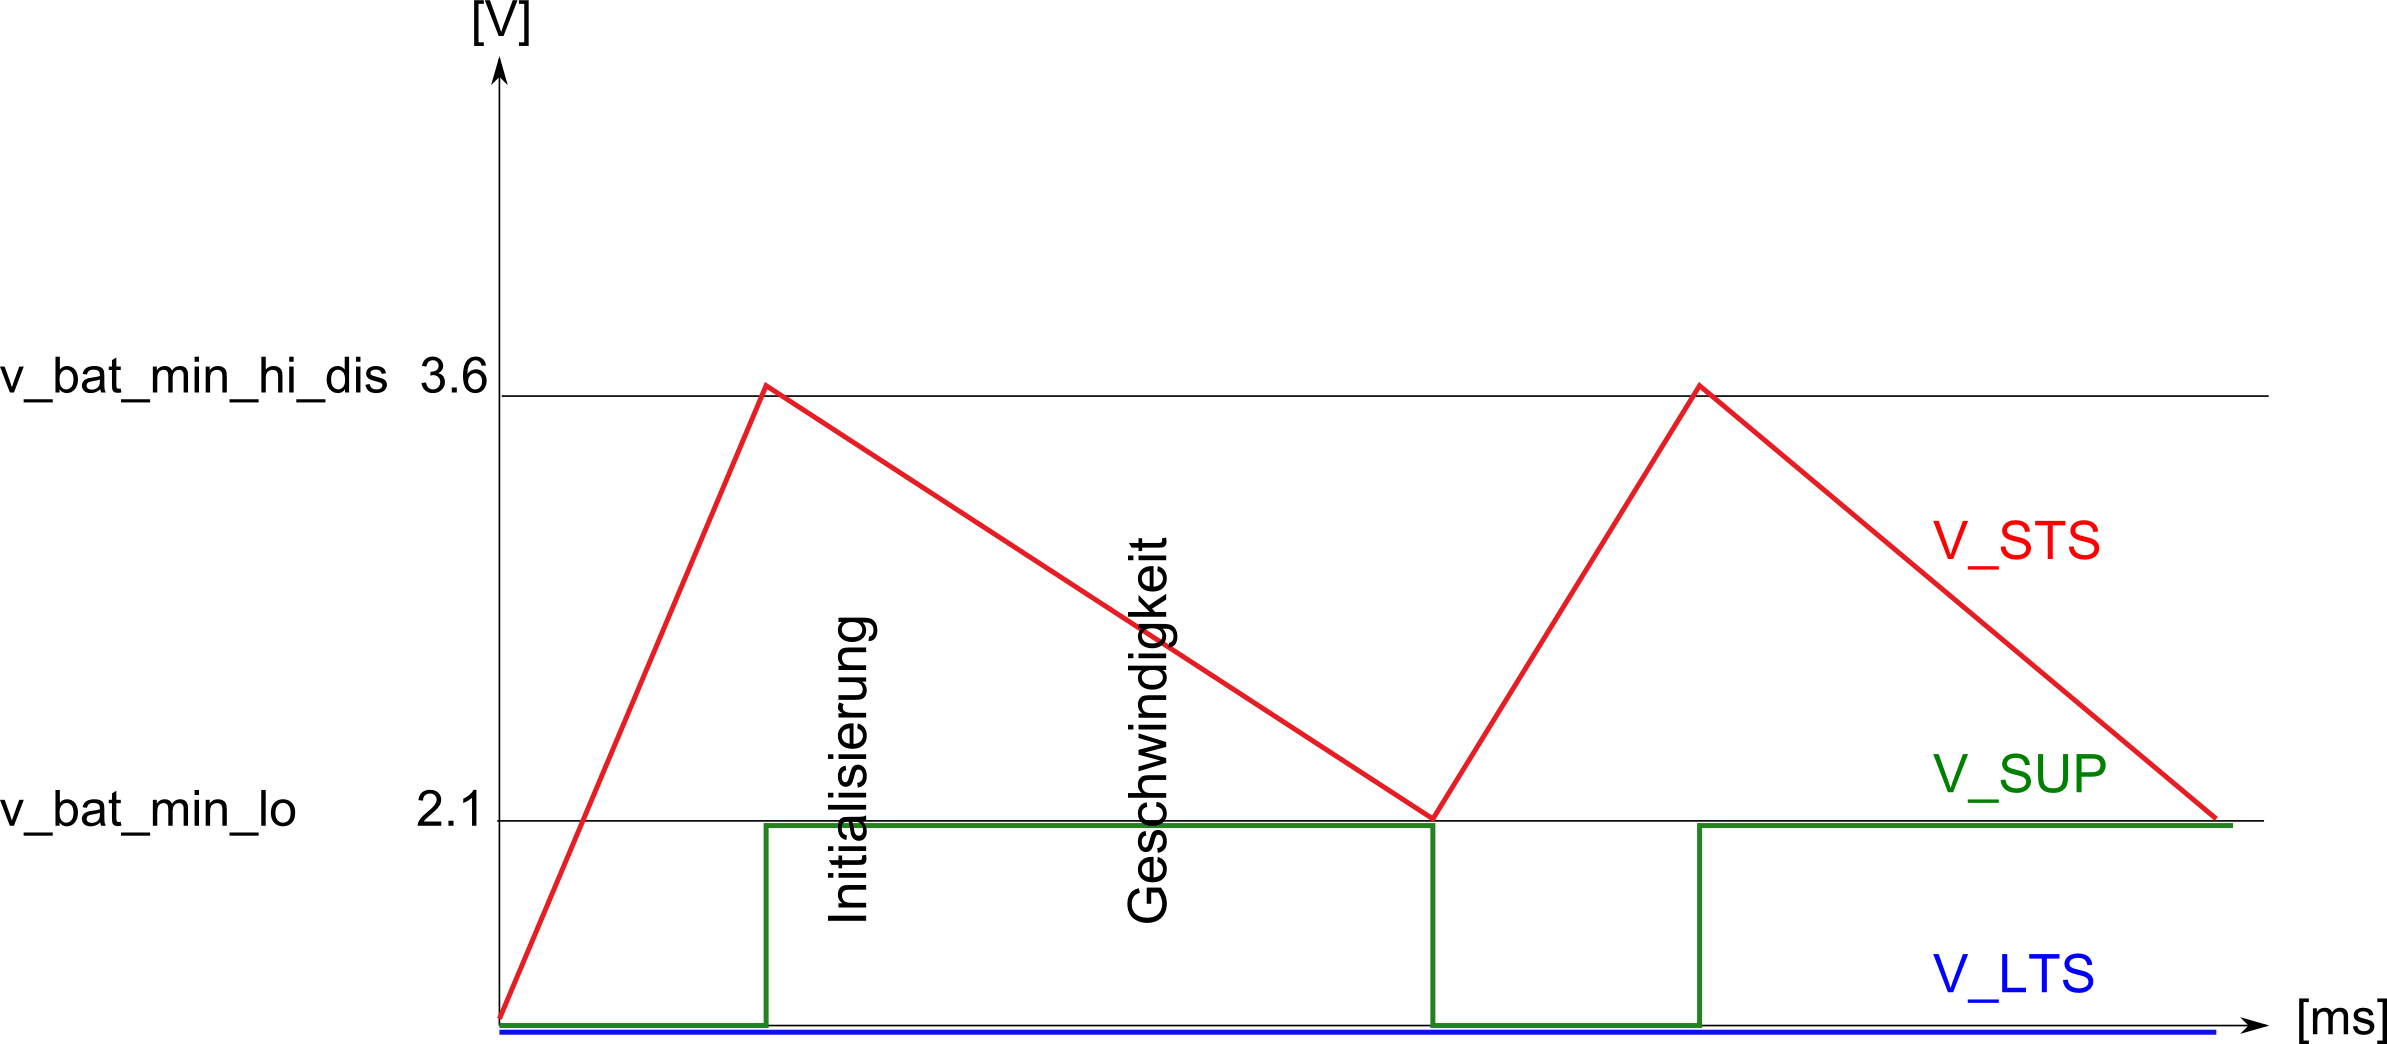
\includegraphics[width=1.0\textwidth]{3Vorgehen/imag/LOW_ENERGY.png}
  \caption{Aktionen bei LOW ENERGIE}
  \label{LOW_ENER}
\end{figure}

Bei etwas mehr Energie befindet sich das System in einem Zwischenzustand (Abbildung \ref{MID_ENER}). Zu jeder Geschwindigkeitsmessung wird ein Sensor ausgelesen. Im Idealfall unterstützt LTS die Stabilität. Wenn nicht, schaltet V\_SUP bei zu wenig Energie ab.

\begin{figure}[ht]
  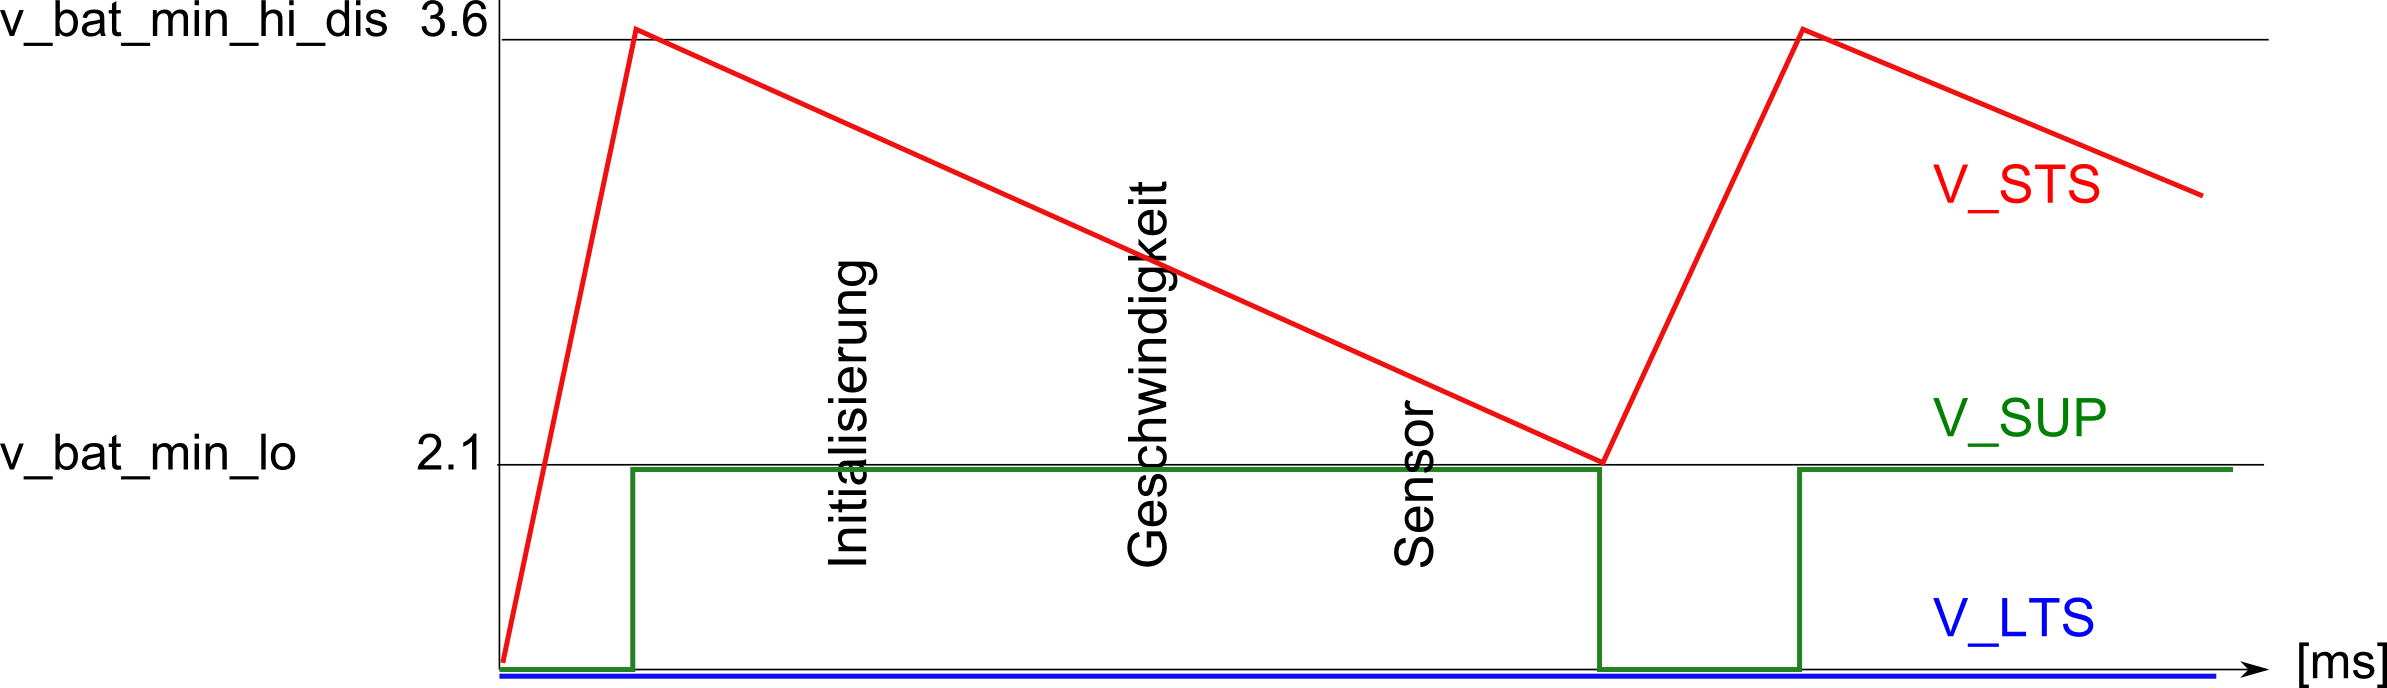
\includegraphics[width=1.0\textwidth]{3Vorgehen/imag/MIDDLE_ENERGY.png}
  \caption{Aktionen bei MIDDLE ENERGIE}
  \label{MID_ENER}
\end{figure}

Im hohen Energiezustand wird mit jedem Geschwindigkeitspaket die aktualisierten Werte der drei Sensoren mitübertragen. 

\begin{figure}[ht]
  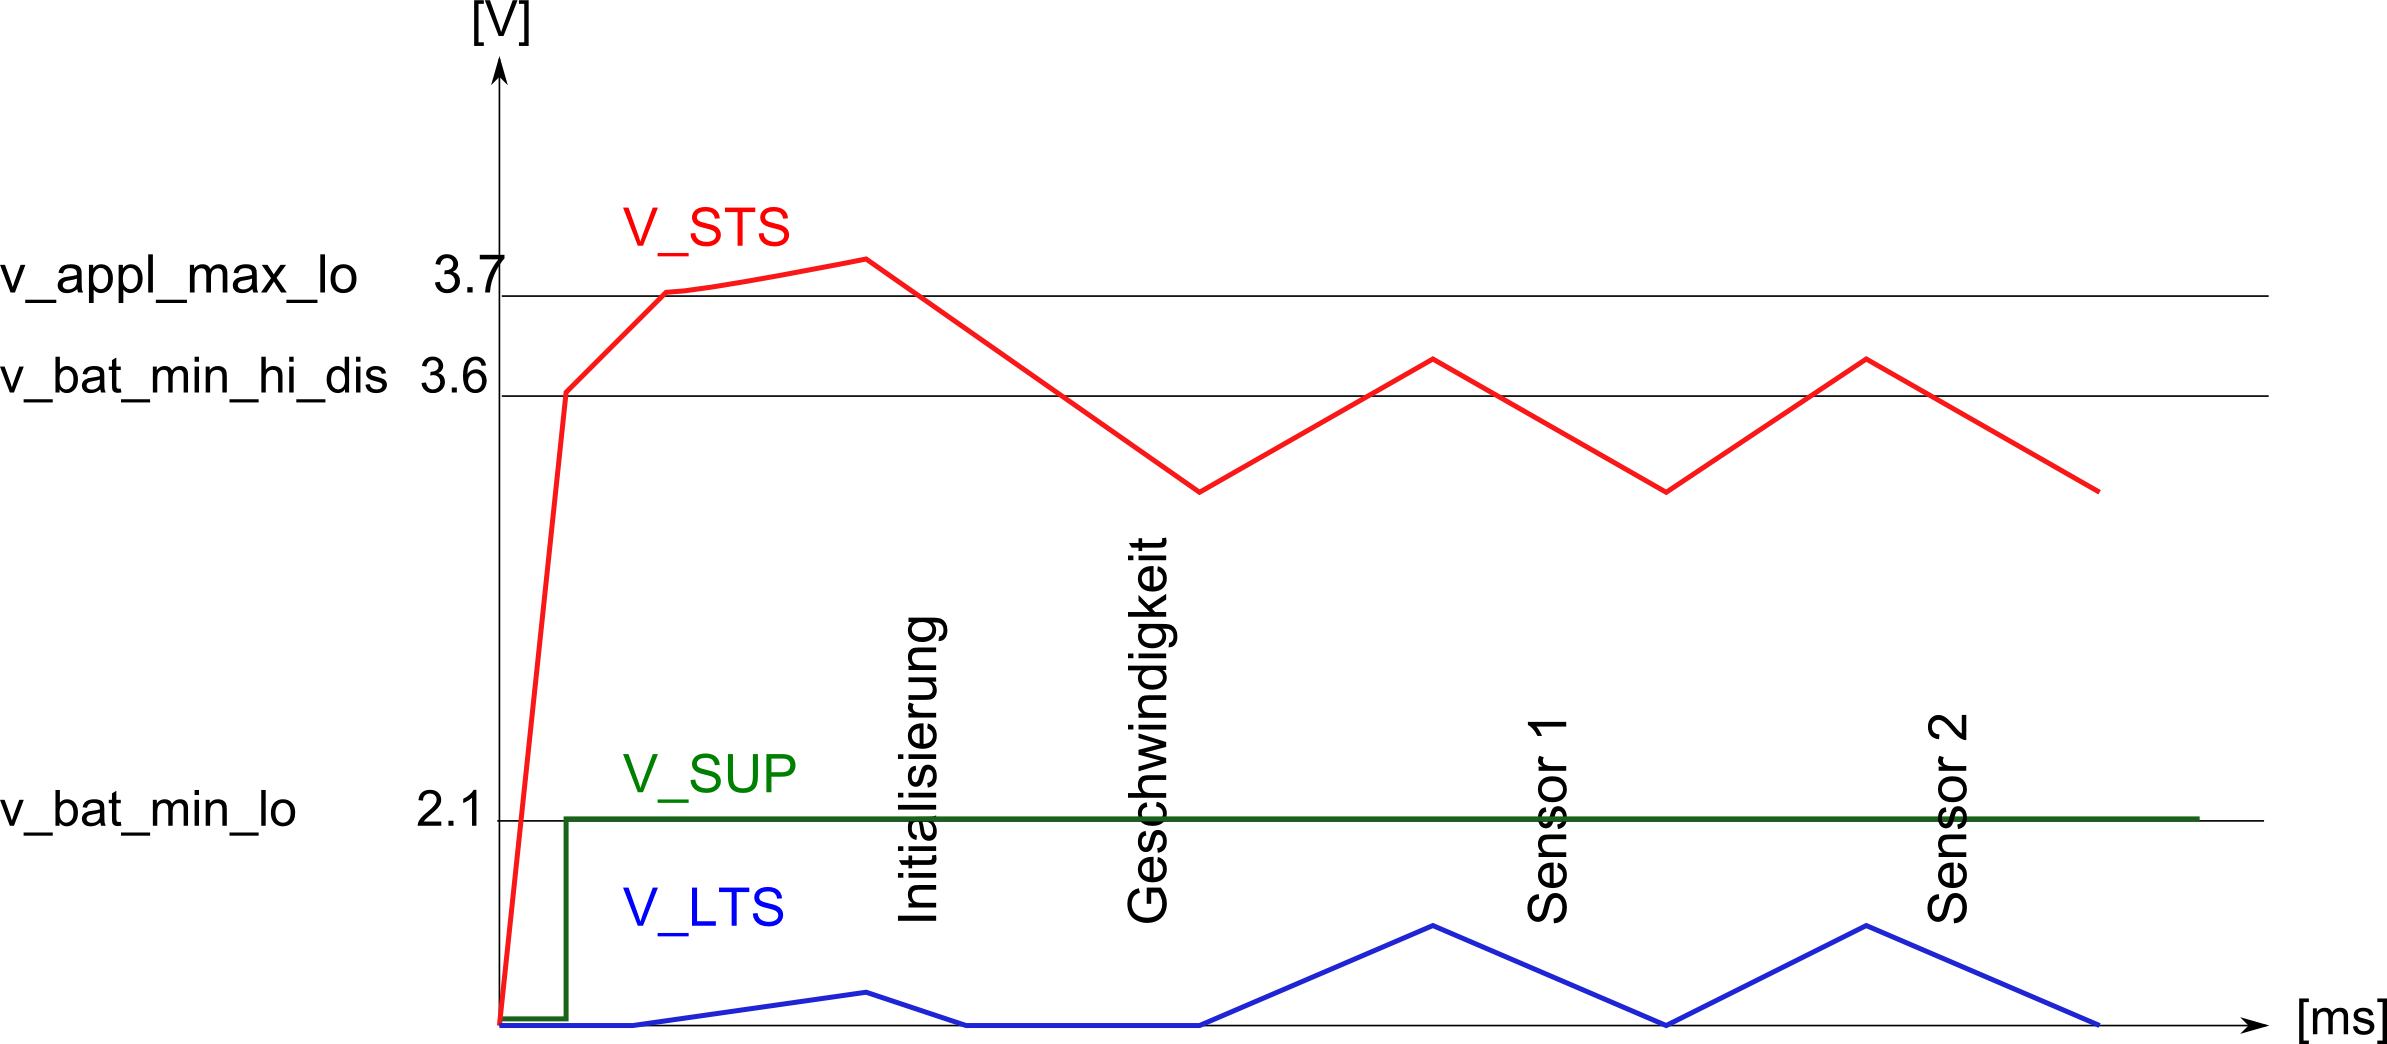
\includegraphics[width=1.0\textwidth]{3Vorgehen/imag/HIGH_ENERGY.png}
  \caption{Aktionen bei HIGH ENERGIE}
  \label{HIGH_ENER}
\end{figure}

%\subsubsection*{Energiezustände umgesetzt in Software}






 4---------------------------------------------------------------------------
\section{Power Management}
\label{powerOptimierung}

Die Verwendung des TI-SensorTags wurde zur Herausforderung. Im ersten Unterkapitel \ref{keinROTS} wird beschrieben, warum die Code-Beispiele von Texas Instrument für den Bicycle Computer nicht verwendet werden können und was dies für die Entwicklung der Applikation bedeutet. In nächsten Unterkapitel \ref{PowerDomains} wird das selektive Ausschalten der Peripherie erklärt und in den letzten zwei Unterkapitel die Umsetzung, wie Schlafenszeiten zwischen den Funktionen eingebaut werden \ref{sleep_funktion} oder wie Funktionen zwischendurch zum Schlafen gezwungen werden (\ref{sleep_while}).



\subsection{Programmieren ohne RTOS}
\label{keinROTS}

Das ausgewählte TI-SensorTag ist für Low Power-Anwendungen ausgelegt. Die Low Power-Programmbeispiele von TI basieren auf RTOS. Da bei 10 km/h Energie, im $\mu$J-Bereich zur Verfügung steht, und die minimale RTOS-Anwendung, die auf TI-SensorTag vorinstalliert ist, Energie von xxJ benötigt, sind Programmlösungen ohne RTOS notwendig. Die Funktionen der Software werden deshalb von Grund auf aufgesetzt. Die Verwendung zur mitgelieferten TI-SensortTag Library ist unabdingbar, da das Memory Mapping nur über die Library zugänglich ist. 

\todo{Energiemessung RTOS}

Das Erschwert die Softwareentwicklung durch folgende drei Punkte

\begin{enumerate}
    \item Es bestehen keine Codebeispiele ohne RTOS. Weder für das Power-Handling, wie die CPU oder eine Peripherie zum Schlafen schicken, noch zur Initalisierung des Systems, dem Auslesen der Sensoren, der Kommunikation per I2C oder SPI, noch zum Verwenden der Timer.
    \item Der Umfang mitgelieferte Library von Texas Instruments (cc26xxware/driverLib) ist enorm. Die Library baut auf impliziten Bezügen für ein optimiertes RTOS auf. Interrupts werden z. B. nicht direkt verarbeitet, sondern gehen über eine der zwei Event Fabric mit diversen Subscribers (\cite{Sensortag_Manual}, S. 238ff) komplex abgehandelt. In der Library sind predefined Funktionen für das RTOS implementiert. Der Versuch, diese predefinierten Funktionen zu verstehen, scheitert an der Komplexität der Library und dem RTOS-Fokus. Durch try and error können Abläufe rekonstruiert werden.
   \item Hat man durch try and error ein lauffähiges Programm entwickelt, ist dies oft nicht lanfristig sicher. Die ist, weil eine gute Dokumentation fehlt. Durch das Einbauen neuer Anforderungen, wie z. B. die Verwendung einer neuen Power Domain oder eines neuen Interrupts, kann das System ungewollt beeinflussen. Jede Erneuerung in der SensorTag-Version verusachte deshalb Nebeneffekte. Der Fortschritt im Programmieren bleibt trotz Klarheit der Umsetzung harzig.
\end{enumerate}

\subsection{Power Domains beim TI-SensorTag}
\label{PowerDomains}

In der Library des TI-SensorTags spielt das Ein- und Ausschalten der 10 Power Domains eine zentrale Rolle (siehe cc26xxware/sys\_ctrl.h, cc26xxware/pwr\_ctrl.h, cc26xxware/prcm.h). Die Abbildung \ref{a_supply} im Anhang \ref{anhang_sensortag_supply} zeigt, die 10 Power Domains. Das TI-SensorTag unterscheidet zwischen drei Always On (AON) Power Domains und CPU, MCU, RFCORE und weiteren Power Domains. Die zweite Abbildung \ref{a_powerdomain} im Anhang \ref{anhang_sensortag_PowerDomain} zeigt die Verstrickung unter den Power Domains. Ausser den zwei generellen Bildern und dem Beschreiben der Registerbits im PRCM-Register ist zu Power Domains nichts dokumentiert (siehe Technical Manual Kapitel 6 Power, Reset, and Clock Management \cite{Sensortag_Manual}, S. 412 - 473).

Wie im oberen Unterkapitel erwähnt, gehen die Entwickler vom Gebrauch des RTOS und den dazugehörenden Funktionen aus. Die Entwickler nehmen der Programmiererin bzw. dem Programmierer die Hintergrundsarbeit ab. Sie kümmerten sich durch das Aufsetzen der Library um die Abhängigkeiten unter den Power Domains. 

Die tieferen Abhängigkeiten viel das erste Mal beim Aufsetzen der Interrupts zum Einlesen des Reed-Switches über die GPIO auf. Vor dem Aktivieren der GPIO-Power Domain funktionierte der interne RTC einwandfrei. Auf Tastendruck konnte nach dem Ablauf der eingestellten Zeit ein BLE-Paket versendet werden. Nachdem der GPIO-Interrupt aktiviert ist, funktioniert der RTC nicht mehr. Nachlesen im Technical Manual ergaben, dass das TI-Sensortag über die Interrupts eine Event Fabric mit zwei Unterabteilungen eingebaut hat. Das Koordinierte Ein- und Ausschalten dieser zusätzlichen Struktur wird nun behandelt. Nach dem dieses Zusammenspiel funktioniert, stellt sich heraus, dass bei schnellen Reed-Switch-Impulsen, ein Problem im Zusammenspiel mit dem Radio-Aufwachen entsteht. Und so weiter und so fort. In den Sitzungsprotokollen xxx  sind die entstandenen Herausforderungen dokumentiert. Die letzte, bis zur Abgabe der Bachelorarbeit noch nicht gelöste Aufgabe, ist das Forcieren des Schlafen während dem Aufstarten eine Sensors. 

Die von aussen nicht einfach durchschaubaren Abhängigkeiten sind der Grund, dass in der TI-Sensortag Version V3 die Power-Optimierung besser war, als dann in der Version V4. Teilweise muss, damit eine Peripherie wie z. B. I2C läuft, mehrere Domains eingeschalten werden. Wenn die Funktionalität läuft, wird versucht, die aktive Zeit zu verkürzen.


\subsection{Schlafenszeiten zwischen Funktionen}
\label{sleep_funktion}

Einfach zu implementieren sind ganze Schalfzyklen nach einem Funktionsblock. Ist eine Aufgabe getätigt, wie z. B. das Starten einer Clock Domain der AON oder das Starten eines Sensors, kann das System schalfen gehen. Dieses Prozedere funktioniert einwandfrei und sicher. Das System wacht aufgrund eines Interrupts wieder auf. Nachfolgend sind die zwei Hauptfunktionen: Vorbereiten zum Stand By (\ref{vorbereiten}) und Ausschalten des Hauptprozessors (\ref{ausschalten}) abgebildet.

\subsubsection{Stand By Prozedur}
\label{vorbereiten}

\todo{als Code markieren, Einrückungen falsch}
Bevor der Prozessor schalfen geht, muss das Recharge Intervall aufgesetzt werden. Während der Prozessor schläft, bleiben Takte der Always On (AON) Power Domain wach wie auch Interrupts dieser Domaine. Zusätzlich werden die Registereinstellungen über das Recharge Intervall am Leben erhalten. 
 
void go\_to\_standby()\{ 
                \linebreak 
	    powerDisableXtal(); \linebreak 
	    powerDisableRFC(); \linebreak
	    OSCHfSourceSwitch();                    // activates lower clock \linebreak
	    powerDisableAuxForceOn(); \linebreak
	    powerEnableMcuPdReq(); \linebreak
	    powerDisableCache(); \linebreak
	    powerDisableCacheRetention(); \linebreak
	            \linebreak
	    // calculate next recharge time \linebreak
	    SysCtrlSetRechargeBeforePowerDown(XOSC\_IN\_HIGH\_POWER\_MODE);   \linebreak     
	    SysCtrlAonSync(); \linebreak
                \linebreak
} \linebreak
	    

\subsubsection{Abschalten}
\label{ausschalten}

\todo{als Code markieren}

void go\_to\_deep\_sleep()\{ 
        \linebreak 
	    powerDisableCPU();\linebreak
	    PRCMDeepSleep();\linebreak
	    SysCtrlAonUpdate();\linebreak
	    SysCtrlAdjustRechargeAfterPowerDown();\linebreak
	    SysCtrlAonSync(); \linebreak
                \linebreak
} \linebreak

	    

	    

\subsection{Schlafenszeiten erzwingen beim Aufwachen der Sensoren}
\label{sleep_while}

Aufgrund der Energiemessungen wird klar, dass die 

Sensor aktivieren

warten

Problem







% 5 ---------------------------------------------------------------------------
\section{Applikationsentwicklung}
Nachfolgend wird der Aufbau von TI SensorTag zusammen mit unserem selbst entwickelten Board als Sensor benannt und die Android Applikation auf dem Smartphone wird einfach als Applikation benannt.

\subsection{Aufbau der Applikation}

Bild einfügen

%\begin{figure}[ht]
%    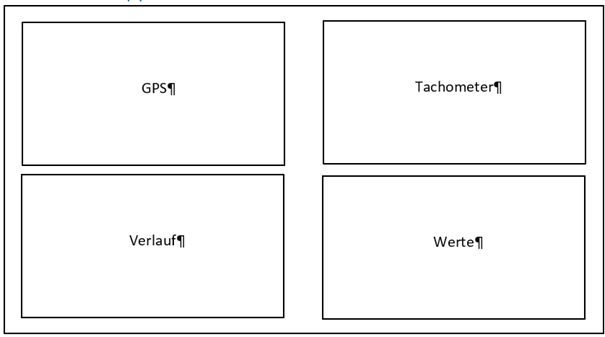
\includegraphics[width=0.5\textwidth]{3Vorgehen/imag/Aufbau_Applikation_erste_Version.PNG}
%    \caption{Aufteilung des Bildschirms}\label{aufbau_applikation_1} 
%\end{figure}

Der Aufbau der Applikation soll Anfangs in vier Teile des Bildschirms geteilt werden. 
Im Bereich GPS soll eine Karte angezeigt werden, ausserdem soll es möglich sein die Route aufzuzeichnen und abzuspeichern.
Der Verlauf zeigt die Entwicklung der Geschwindigkeit über einen gewissen Zeitraum, wobei es wählbar sein soll welche Daten angezeigt werden.
Die Geschwindigkeit soll anschaulich in einem Tachometer angezeigt werden und die Tachonadel soll im besten Fall animiert sein.
Im Bereich der Werte sollen die aktuellen Werte in Zahlen und den entsprechenden Einheiten dargestellt werden.
Schnell wurde klar, dass dieser Aufbau wenig Sinn macht, da die Bereiche auf einem Smartphone viel zu klein wären und nicht mehr leserlich sein würden. Darum wurde ein neues Konzept erarbeitet, welches in der Abbildung x ersichtlich ist.

\subsubsection{Home-Screen}

Als erstes soll der Benutzer den sogenannten Home-Screen sehen, hier werden der Tachometer, die Werte und ein paar Buttons angezeigt. Je nach Anzahl der Funktionen sollen neue Buttons implementiert werden. So soll beispielsweise für die Sensorwahl ein Button vorhanden sein. Während der Entwicklung der Applikation wurde die Idee von einer GPS-Karte und einem Verlauf ebenfalls verworfen, da diese Funktionen aus zeitlichen Gründen nicht mehr realisierbar waren. Jedoch wäre der Home-Screen in der Lage mehr Buttons aufzunehmen, es muss nur darauf geachtet werden, dass die Anzeige der Werte nicht zu gross wird.

\subsubsection{Sensorwahl}

Schnell wurde klar, dass die Auswahl eines spezifischen Sensors wichtig werden würde, für den Fall, dass einmal mehrere Sensoren vorhanden wären. Ein Beispiel, würde unsere Applikation bei einem Fahrradrennen eingesetzt werden, so müsste die Applikation auf dem Smartphone mit dem Sensor am Fahrrad gepaart werden. Ansonsten würde man die Daten von allen Sensoren empfangen und die Anzeige würde nicht die Daten des eigenen Sensors anzeigen.

\subsubsection{Einheiten und Einstellungen}

Es kam ebenfalls der Wunsch auf, die Einheiten der Werte, einstellbar zu machen, da die Applikation bestenfalls auch in anderen Ländern verwendet werden soll. Also wäre es optimal, wenn die Geschwindigkeit beispielsweise auch in Miles per Hour dargestellt werden könnte. Vielleicht müsste auch eine Einstellungsmöglichkeit bereitgestellt werden, damit die Temperatur kalibriert werden kann.

\subsubsection{BLE-Kommunikation}

Der wichtigste Teil der Applikation ist die Bluetooth-Kommunikation, hier werden die Daten vom Sensor empfangen. Die Daten müssen nach dem Empfangen gefiltert werden, damit sichergestellt wird, das die empfangenen Daten von einem unserer Sensoren kommen. Sobald sichergestellt ist, das die empfangenen Daten zu unserem Sensor gehört, müssen diese umgerechnet werden.

\subsubsection{Inbetriebnahme des Codes der PA}

Als erster Schritt wurde der Code der vorangegangenen Arbeit analysiert und die wichtigen Teile zur Bluetoothkommunikation übernommen. Es wurden folgende Funktionen aus dem Code übernommen: onStart, onActivityResult, scanLeDevice, BluetoothAdapter.LeScanCallback.

Die Funktion onStart wurde in BLE\_init umbenannt und der Mechanismus zum Wachhalten des Geräts wurde entfernt. Der Mechanismus wurde entfernt, da dieser nicht mehr funktionierte. Ebenfalls wurde die Funktion in die Funktion onCreate eingefügt, um den Code übersichtlicher zu gestalten und da diese Funktion nur einmalig aufgerufen werden musste.
 
Die Methoden onActivityResult und scanLeDevice wurden komplett übernommen.

Die Callback-Funktion des Bluetoothadapters BluetoothAdapter.LeScanCallback wurde strukturell übernommen, jedoch wurde die Codierung zur Verarbeitung der Daten entfernt.

\subsubsection{Filter einbauen}
Der nächste logische Schritt war, dass die empfangenen Daten gefiltert werden mussten. Dafür wurde folgende Struktur definiert, damit festgestellt werden kann, ob die Daten von einem unserer Sensoren versendet wurden.

\begin{tabbing}
   Length	\quad\= Type	\quad\= UUID 	\quad\= Package ID	\quad\= Speed	\quad\= Pressure	\quad\= Temperature	\quad\= Humidity	\quad\= Checksum   \\[0.8ex]
   23	\> 0x03	\> 0xDEBA \> 2 bytes\> 4 bytes\> 4 bytes\> 4 bytes\> 2 bytes \\
\end{tabbing}
Aufgrund dieser Struktur können alle empfangenen Daten, welche nicht die definierte Länge, Typ und UUID besitzen, ignoriert werden.

Wenn sichergestellt ist, dass die Daten von unserem Sensor stammen, musste noch die Adresse vom Sender gespeichert werden. Alle Adressen werden in einer Liste gespeichert, vor dem Speichern wird jedoch noch geprüft, ob die Adresse bereits in der Liste ist, falls ja wird die Adresse nicht noch einmal gespeichert.

\subsubsection{Berechnung der Daten}

Der Sensor sendet Werte, wie den Zeitunterschied zwischen zwei Magnetdurchläufen, dem Luftdruck, der Temperatur und die relative Luftfeuchtigkeit. Diese Daten müssen erst noch in die realen Werte umgerechnet werden, da alle Werte in mehreren Bytes verteilt vorliegen.

Der Zeitunterschied zwischen zwei Magnetdurchläufen wird in vier Bytes dargestellt. Die ersten beiden Bytes enthalten die Anzahl Sekunden, es muss also das erste Byte um acht Bit geschoben werden und anschliessen muss das zweite Byte noch addiert werden. Folgende Formel zeigt die Umrechnung von zwei Bytewerten in eine reelle Zahl:

\begin{equation}
	t = ((byte_0 << 8) + byte_1)
\end{equation}

Die erhaltene Zahl muss noch mit einem Typecast in den Datentyp float umgewandelt werden.

Das dritte und vierte Byte des übermittelten Zeitunterschieds enthält die Sekundenbruchteile. Folgende Formel zeigt, wie die Bytes verrechnet werden müssen, um die korrekten Werte zu erhalten:

\begin{equation}
	t = \frac{((byte_2 << 8) + byte_3)}{2^{16}}
\end{equation}

Der erhaltene Sekundenbruchteil kann nun zu den ganzen Sekunden dazu addiert werden, um die ganze Zeit zwischen zwei Magnetdurchläufen zu erhalten.

Ein Beispiel, wird also der hexadezimale Wert 0x00014000 empfangen sind das 1.25 Sekunden zwischen zwei Magnetdurchläufen.

Um die Geschwindigkeit zu erhalten muss der Radumfang durch die erhaltene Zeit geteilt werden. Jedoch befinden sich an unserem Rad zwei Magnete, deswegen darf nur der halbe Radumfang verrechnet werden. Ausserdem ist das Resultat in m/s und muss deshalb noch in km/h umgerechnet werden, was nichts anderes als eine Multiplikation mit dem Faktor 3.6 ist.

Der Druck wird in Pa übertragen, hier müssen die verschiedenen Bytes miteinander addiert werden und in hPa umgerechnet werden. Es werden jedoch nur die letzten drei Bytes mit Werten befüllt sein, das erste Byte kann ignoriert werden. Folgende Formel zeigt die Umrechnung der Bytes in eine float Zahl.

\begin{equation}
	p = (float)((byte_2 << 16) + (byte_1 << 8) + byte_0) * 0.01
\end{equation}

Die barometrische Höhenformel zeigt die Abhängigkeit des Druckes von der aktuellen Höhe.

\begin{equation}
	p(h) = p_0 * e^{-\frac{h}{7991 m}}
\end{equation}

- Referenz: Buch "Mathematik für Ingenieure und Naturwissenschaftler Band 1, 12. Auflage, Lothar Papula, Seite 284

Durch Umformen ergibt sich die folgende Formel, womit sich die Höhe aus dem Druck berechnen lässt.

\begin{equation}
	h = ln(\frac{p(h)}{p_0}) * (-7991 m) = ln(\frac{p(h)}{1013.25 hPa}) * (-7991 m)
\end{equation}

Die Temperatur wird in zwei Bytes übertragen. jedoch wird die Temperatur nicht in $^\circ$C übertragen, sondern in Tausendsteln. Das bedeutet die Temperatur, welche empfangen wird, muss zusammengesetzt und mit 1000 dividiert werden. Die Formel sieht folgendermassen aus:

\begin{equation}
	T = (float)((byte_1 << 8) + byte_0) * 0.001
\end{equation}

Der letzte Wert, welcher vom Sensor versendet wird, ist die relative Luftfeuchtigkeit. Die Formel zur Berechnung der relativen Luftfeuchtigkeit sieht folgendermassen aus:

\begin{equation}
	H = (float)(byte_3 << 24) + (byte_2 << 16) + (byte_1 << 8) + byte_0
\end{equation}


\subsection{Einstellungsmöglichkeiten}

Als nächstes wurde die Aufgabe in Angriff genommen, die Applikation als User einstellen zu können. Es musste genau überlegt werden, welche Einstellungen ein User machen darf und welche dem Programmierer, bzw. der Applikation überlassen werden.

\subsubsection{Adressauswahl}

Die Adressauswahl, oder auch Sensorwahl, wurde bald ein Bedürfnis, da der User die Applikation mit seinem eigenen Sensor paaren können sollte. Es sollte sichergestellt werden, dass die Applikation nach der Sensorwahl nur noch Daten von dem gewählten Sensor anzeigt und die Daten der anderen Sensoren ignoriert werden. Die Adressen von Sensoren in der Nähe sollten aber weiterhin gespeichert werden, damit man gegebenenfalls auch einen anderen Sensor auswählen konnte.

Immer wenn Daten empfangen werden und die Struktur mit der definierten Struktur übereinstimmen soll die Adresse gespeichert werden. Dafür wurde folgende Funktion entwickelt:

\begin{figure}[ht]
    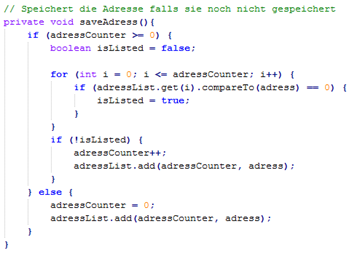
\includegraphics{3Vorgehen/imag/app_saveAdress.png}
    \caption{Sourcecode saveAdress}
	\label{app_saveAdress} 
\end{figure}

Der adressCounter wird mit dem Wert -1 initialisiert, werden die ersten Daten mit der vorgegeben Struktur empfangen wird die Funktion automatisch die Adresse in der adressList an der Stelle 0 speichern. Werten erneut Daten von einem unserer Sensoren empfangen wird zuerst geprüft, ob die Adresse bereits ein Teil der adressList ist, falls die Adresse noch nicht in der Liste enthalten ist, wird der Index, bzw. der adressCounter, erhöht und die Adresse in der Liste gespeichert.

Sobald eine Adresse ausgewählt wurde müssen die zukünftigen Datenpackete überprüft werden, ob sie vom ausgewählten Sensor stammen. Die Funktion checkAdress überprüft, ob die ausgewählte Adresse der Adresse des Sensors entspricht, welche die neuen Daten gesendet hat. Sollte keine Adresse ausgewählt sein, so wird dies genauso behandelt, als ob der Sensor die richtige Adresse hat.

\begin{figure}[ht]
    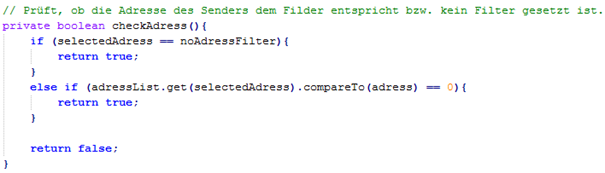
\includegraphics{3Vorgehen/imag/app_checkAdress.png}
    \caption{Sourcecode checkAdress}
	\label{app_checkAdress} 
\end{figure}

Der User muss noch die Möglichkeit haben eine Adresse auszuwählen, dafür wird eine neue Activity erstellt. Die neue Activity ist eine List-Activity, das bedeutet es wird eine Liste von möglichen Adressen angezeigt, welche mit einem Klick auf die gewünschte Adresse ausgewählt wird. Anschliessend wird die ausgewählte Adresse an die Haupt-Activity zurückgegeben. In Abbildung \ref{BLEadressauswahl} ist die List-Activity zu sehen, welche eine Adresse zur Auswahl hat. Damit die ausgewählte Adresse von der Haupt-Activity überhaupt empfangen werden kann musste die List-Activity mit den auszuwählenden Adressen mit folgendem Befehl gestartet werden: startActivityForResult. Die gestartete Activity kann somit ein Resultat, also die ausgewählte Adresse zurückgeben und die Haupt-Activity kann diese in der Funktion onActivityResult empfangen und abspeichern. Die genaue Ausführung der Übergabe der Adressen, sowie die Rückgabe der ausgewählten Adresse kann dem Quellcode entnommen werden.

\begin{figure}[ht]
    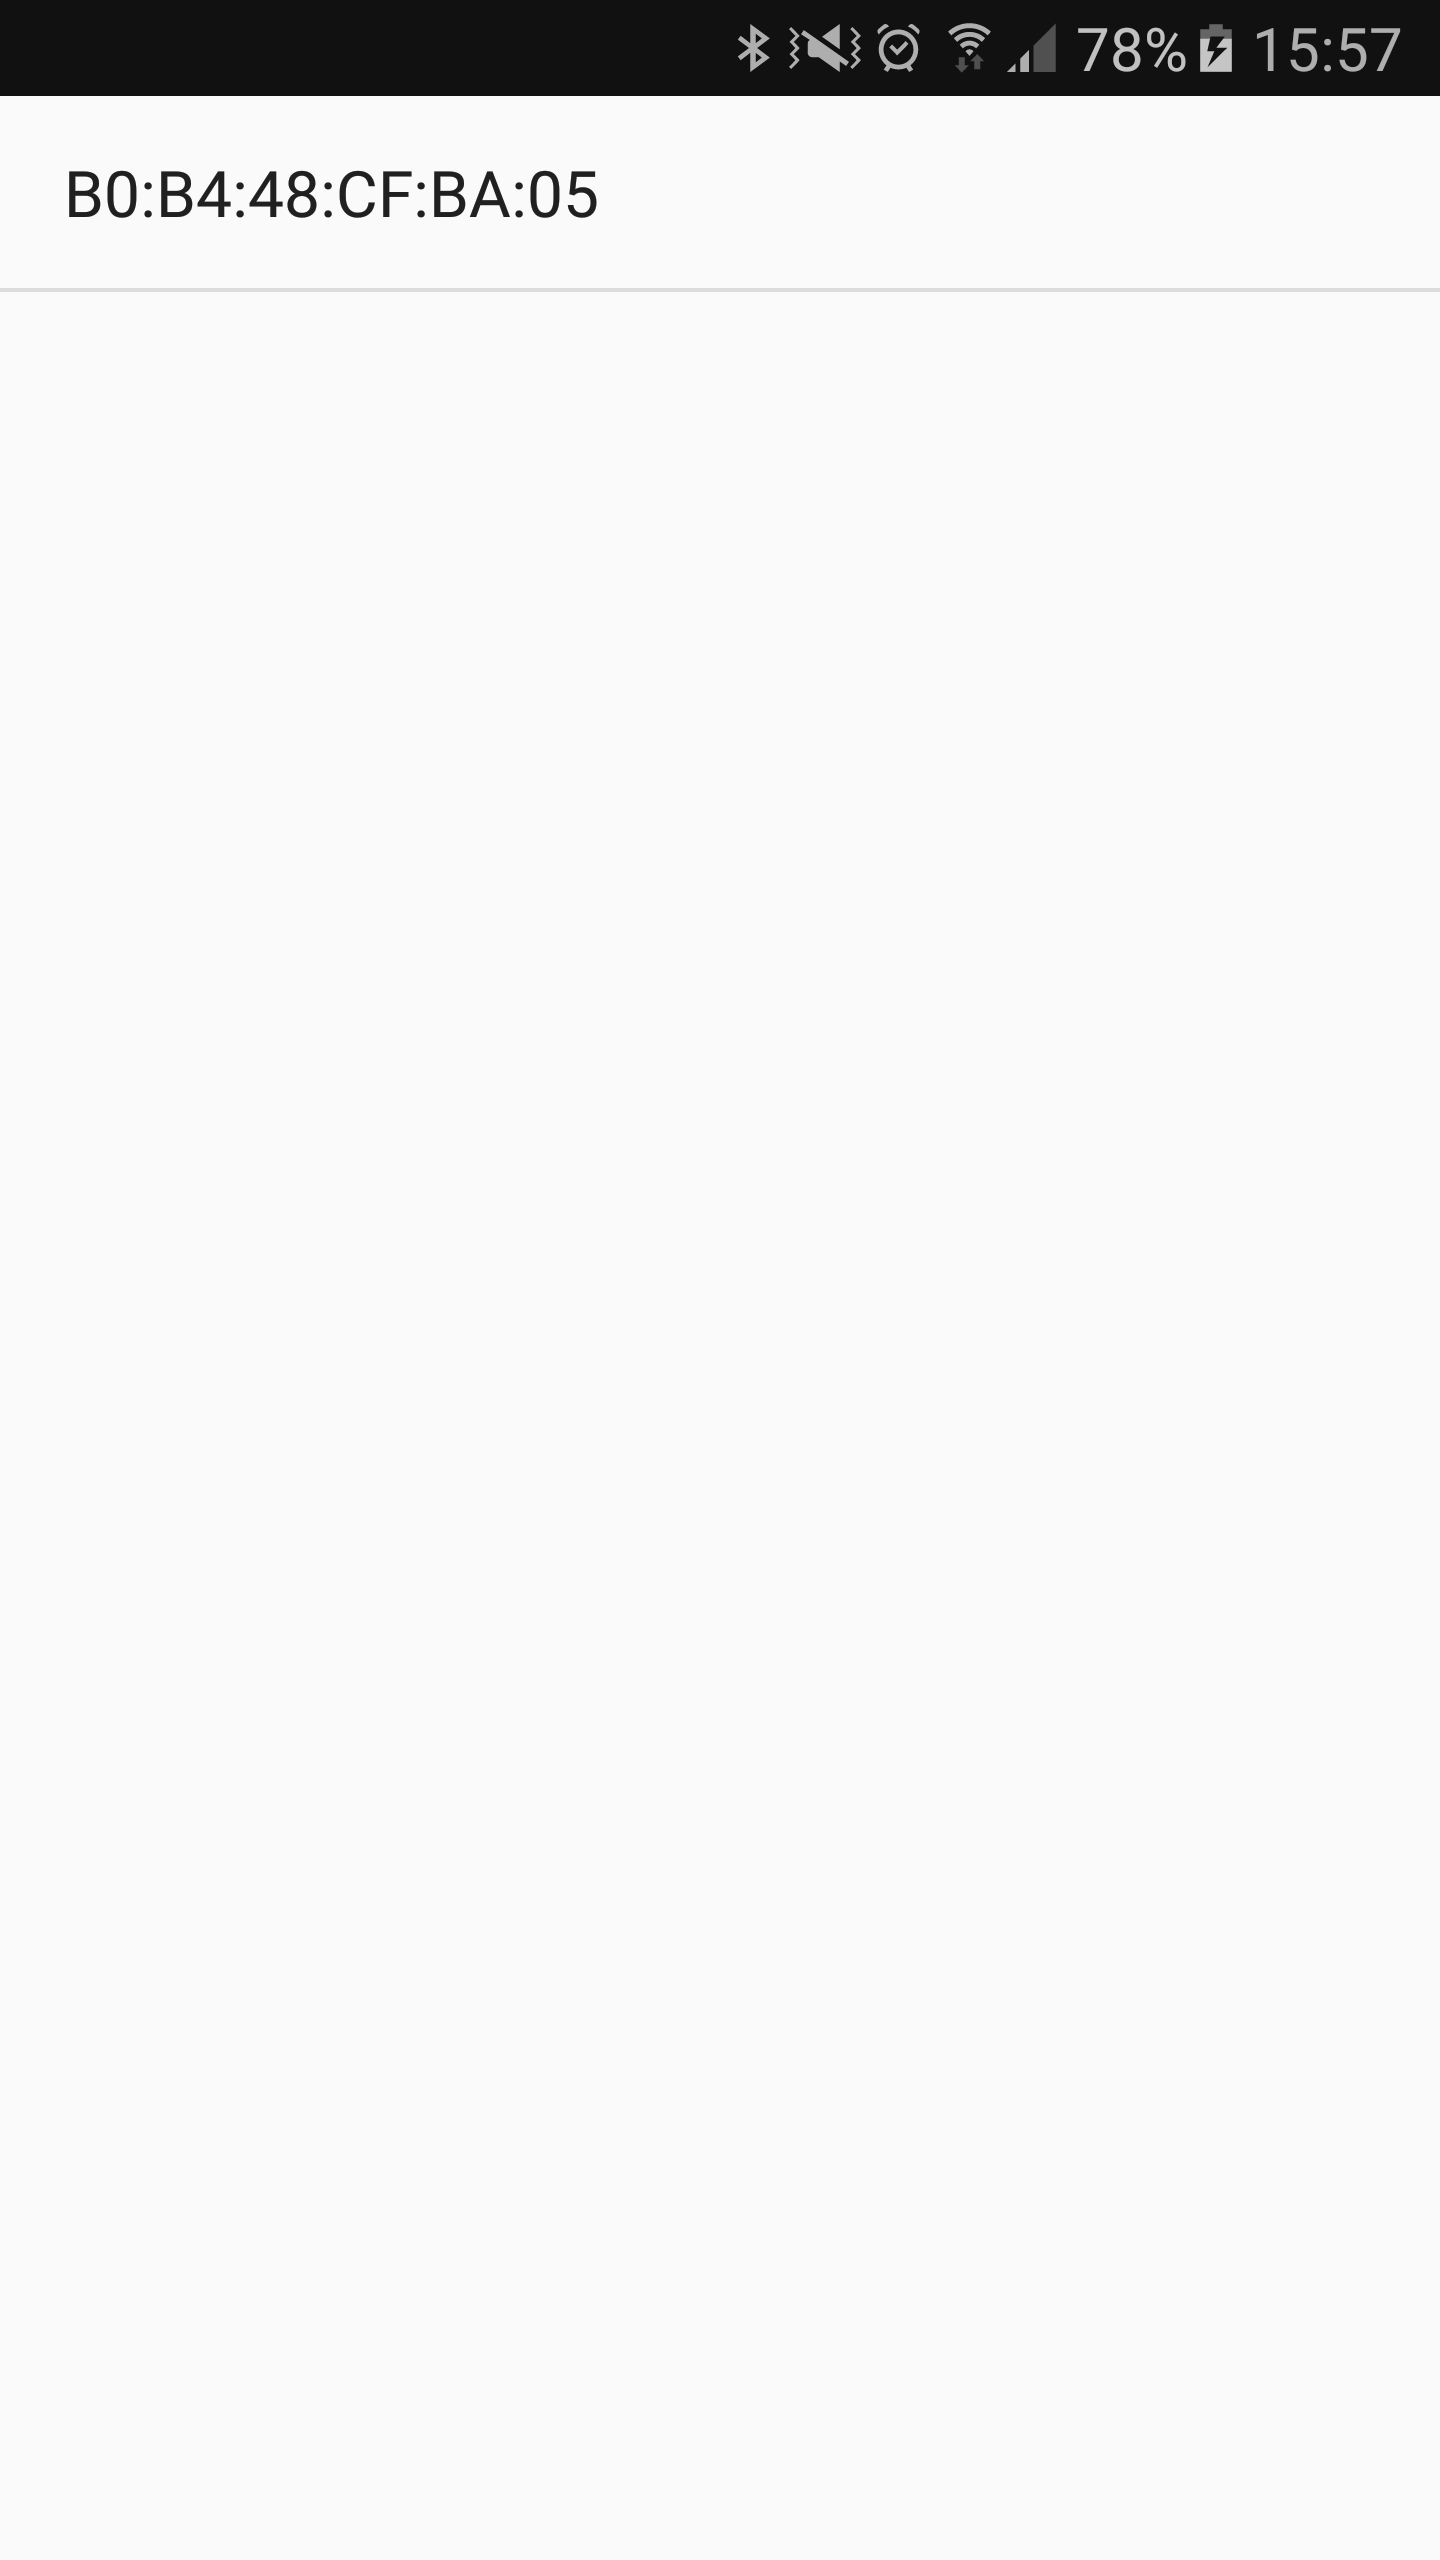
\includegraphics{3Vorgehen/imag/BLEAdresseAuswaehlen.png}
    \caption{Adressauswahl mit nur einer Adresse}
	\label{BLEadressauswahl} 
\end{figure}

\subsubsection{Einheiten}

Die Einheiten der empfangenen Daten sollten ebenfalls einstellbar gestaltet werden. Für diesen Zweck wurden mehrere Enumeration definiert, die Enumeration für die Temperatur sieht folgendermassen aus:

\begin{figure}[ht]
    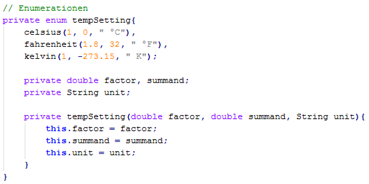
\includegraphics{3Vorgehen/imag/app_tempSetting.png}
    \caption{Sourcecode Enumeration}
	\label{app_tempSetting} 
\end{figure}

Es wurde der Enumeration drei Elemente hinzugefügt, welche alle einen Faktor, einen Offset und einen String mit der geschriebenen Einheit enthalten. Anhand dieser Enumeration kann der Faktor und der Offset einfach zugänglich gemacht werden. 

- Referenz Temperaturumrechnung: %http://www.umrechnung.org/masseinheiten-temperatur-celsius-fahrenheit-kelvin/celsius-fahrenheit-umrechnung.htm (Konsultation am 22.04.16)
- Referenz Druckumrechnung: %http://www.dolder-ing.ch/wissen/Einheiten/Tab_Druckumr/Tab-Druckumrechn-Gebrf.htm (Konsultation am 22.04.16)
- Referenz Geschwindkeitsumrechnung: %http://www.convertworld.com/de/geschwindigkeit/knoten.html (Konsultation am 22.04.16)

Die Enumerationen wurden anschliessend verwendet um die aktuelle Einstellung der Einheiten abzuspeichern. Da die Einstellung der Einheiten nun gespeichert werden konnte, musste diese Einstellung dem User zugänglich gemacht werden.

Eine neue Activity wurde codiert, welche drei Spinner zur Auswahl der Einheiten, einen EditText für die Eingabe des Radumfangs und ein EditText für die Kalibrierung der Temperatur zur Verfügung stellt. Die eingestellten Einheiten und die eingetragenen Werte werden über den Speichern-Button an die Haupt-Activity zurückgegeben. In der onActivityResult Methode in der Haupt-Activity werden die aktuellen Einstellungen empfangen und abgespeichert und anschliessend zur Darstellung der Werte verwendet. Erst bei der Anzeige der Werte, werden die eingestellten Faktoren und Summanden der Enumerationen verwendet.

Abschliessend wurde die Activity zur Einstellung der Einheiten noch dahingehend verbessert, dass die eingestellten Einheiten und die eingetragenen Werte, bei erneutem Aufrufen der Activity dargestellt werden. Wird die Activity zur Einstellung der Einheiten gestartet, wird ihr die aktuelle Einstellung übergeben und die Spinner und EditText zeigen, die zuvor abgespeicherten Werte an. Ein Beispiel, wenn man in der Activity den Spinner für die Temperatur auf "Fahrenheit ($^\circ$F)" einstellt und diese Einstellung abspeichert. Die Activity dann erneut über einen Druck auf den Button startet, wird beim Spinner für die Temperatur die Einstellung "Fahrenheit ($^\circ$F)" angezeigt, da diese Einstellung zuvor abgespeichert wurde.

\begin{figure}[ht]
    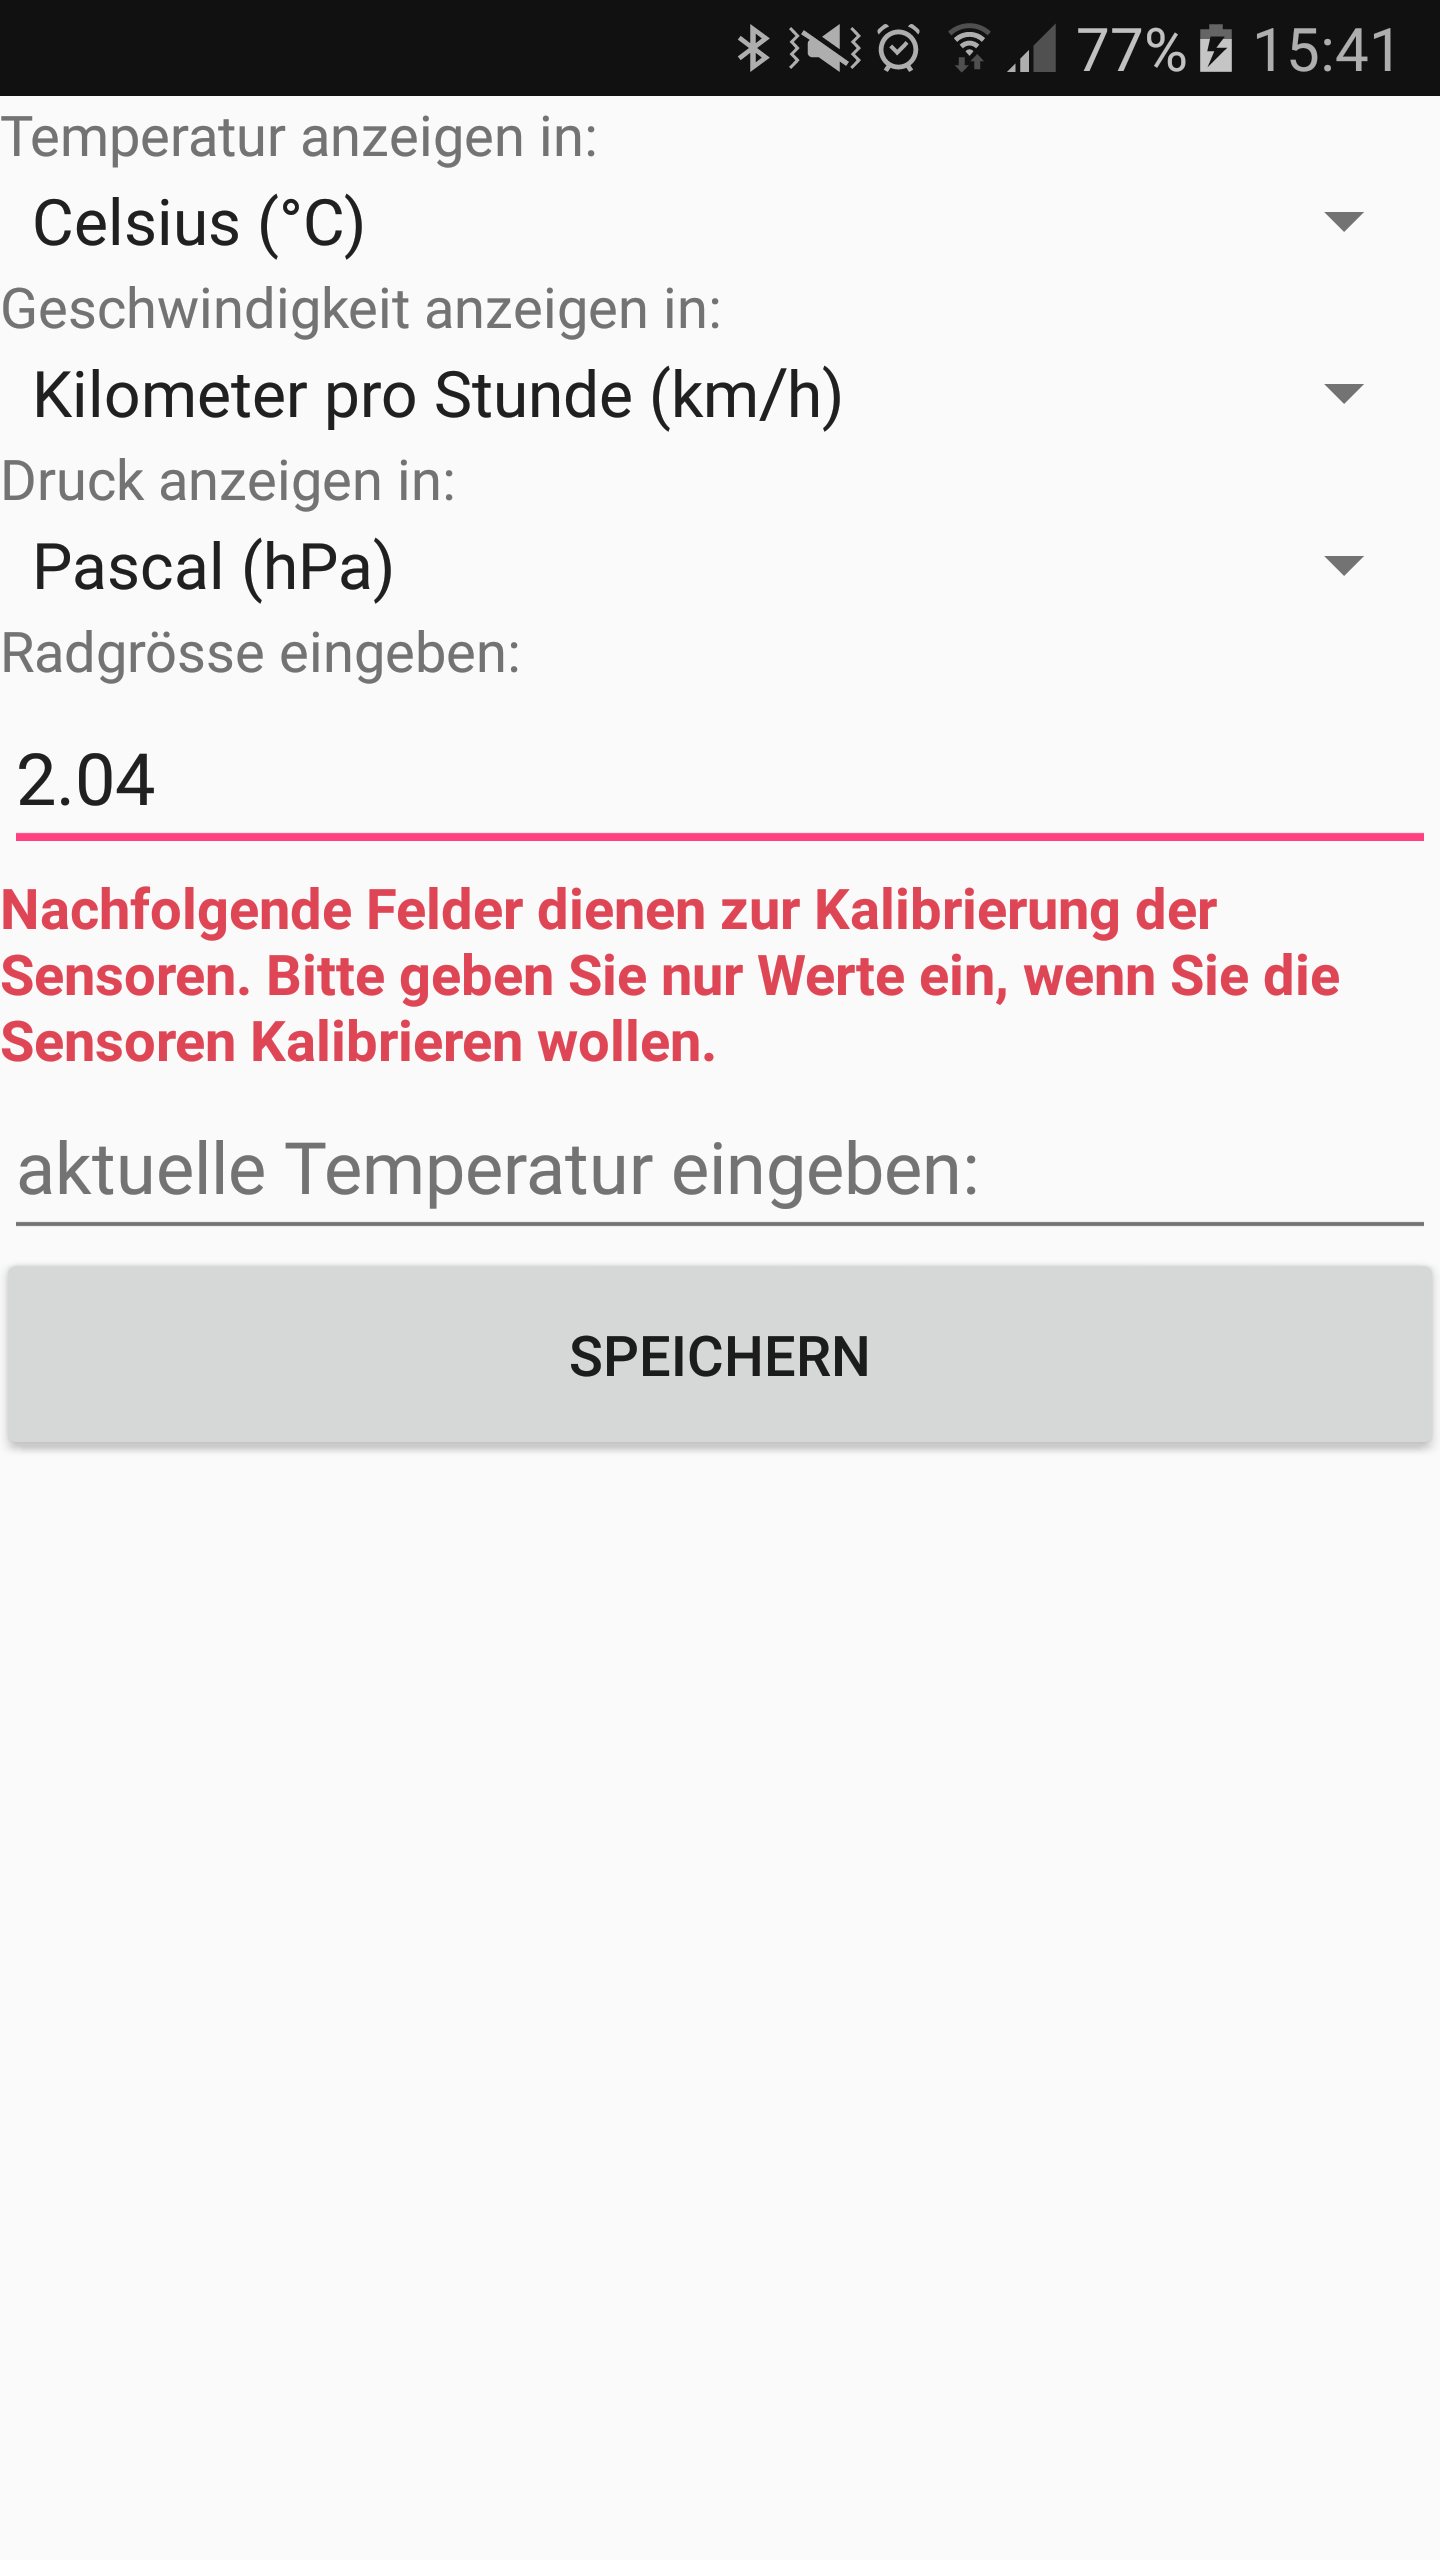
\includegraphics{3Vorgehen/imag/BLEEinheitenUndEinstellungenStart.png}
    \caption{Bildschirm der Einheiteneinstellung}
	\label{BLEEinheitenUndEinstellungenStart} 
\end{figure}

\subsubsection{Kalibrierung}

Während der Entwicklung wurde festgestellt, dass der Wert der Temperatur von der Referenztemperatur abweicht. Aus diesem Grund wurde eine Möglichkeit zur Kalibrierung der Temperatur geschaffen.

Die Kalibrierungsmöglichkeit befindet sich in der gleichen Activity, wie die Einstellungen der Einheiten und der Eingabemöglichkeit für den Radumfang. Wird bei dem Textfeld ein Wert eingegeben, so wird diese Temperatur an die Haupt-Activity zurückgegeben. Die Referenztemperatur wird gespeichert und beim Empfang der nächsten Daten, wird die automatisch ein Offset berechnet. Dieser Offset fliesst automatisch in die Berechnung der Temperatur ein.

\subsection{Animierter Tachometer}

Eine interessante Aufgabe war die Realisierung eines animierten Tachometers, da diese Funktion dem User der Applikation sofort ins Auge stechen würde. Diese Funktion würde die ansonsten relativ triste Aufmachung der Applikation aufwerten. Es sollte ein Tachometer entwickelt werden, welches eine animierte Tachonadel hat, die die aktuelle Geschwindigkeit anzeigt.

\subsubsection{Funktionsweise}

Bereits in der PA von Manuel König wurde mit der Anzeige von Bitmaps experimentiert. Es lag nahe, diese Erfahrung zu nutzen und für dieses Problem eine möglichst einfache Lösung zu generieren. In Android ist es möglich ein Bitmap in ein Zahlenarray zu laden, dieses Array anzupassen und schlussendlich das Array wieder in ein Bitmap umzuwandeln.

Die Funktion drawTacho liest die Pixel eines Bildes eines Tachometers ohne Tachonadel ein, dreht es und fügt die rote Tachonadel direkt in das Bild ein.

%\begin{figure}[ht]
%    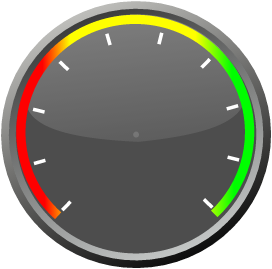
\includegraphics{3Vorgehen/imag/tachometer.png}
%    \caption{Tachometer ohne Tachonadel}
%	\label{tachometer} 
%\end{figure}

Das Bild konnte mit folgender Funktion eingelesen werden:

\begin{figure}[ht]
    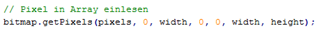
\includegraphics{3Vorgehen/imag/app_getPixel.png}
    \caption{Sourcecode getPixel}
	\label{app_getPixel} 
\end{figure}

Die Bitmap wird in ein eindimensionales Integer-Array eingelesen, die Werte im Array stellen den Farbwert des jeweiligen Pixels dar. Diese Farbwerte können nun verändert werden. Als erstes wurde das ganze Bild gespiegelt, da es noch falsch herum ist, heisst der rote Bereich des Tachometers soll auf der rechten Seite angezeigt werden.

Nach dem Spiegeln des Bildes musste noch die Tachonadel direkt in das Integer-Array eingefügt werden. Die genaue Vorgehensweise wird im nachfolgenden Punkt genauer beschrieben.

Aus dem bearbeiten Integer-Array konnte anschliessend eine Bitmap erstellt werden, welches von der Funktion zurückgegeben wurde. Wichtig ist dabei, dass die richtige Konfiguration ausgewählt wurde, da ansonsten das Bitmap falsch oder gar nicht angezeigt werden konnte.

\begin{figure}[ht]
    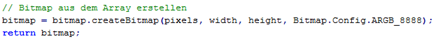
\includegraphics{3Vorgehen/imag/app_createBitmap.png}
    \caption{Sourcecode createBitmap}
	\label{app_createBitmap} 
\end{figure}

\subsubsection{Mathematik der Tachonadel}

\begin{figure}[ht]
    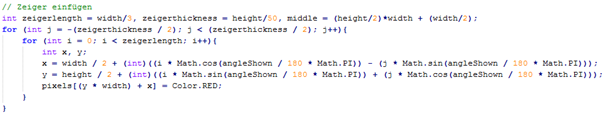
\includegraphics{3Vorgehen/imag/app_drawNeedle.png}
    \caption{Sourcecode Mathematik des Zeigers}
	\label{app_drawNeedle} 
\end{figure}

Die Tachonadel wurde in mehreren Schritten animiert, erst wurde ein Strich mit der Breite von einem Pixel animiert. Die Tachonadel kann als ein Vektor angesehen werden, der im Ursprung gedreht und anschliessend verschoben wurde. Die X- bzw. Y-Koordinaten im Bild konnten folgendermassen berechnet werden:

\begin{equation}
	x = \frac{Breite\, des\, Tachometers}{2} + L\ddot{a}nge\, der\, Tachonadel * \cos(Winkel\, der\, Tachonadel)
\end{equation}

\begin{equation}
	y = \frac{H\ddot{o}he\, des\, Tachometers}{2} + L\ddot{a}nge\, der\, Tachonadel * \sin(Winkel\, der\, Tachonadel)
\end{equation}

Anschliessend sollte die Tachonadel dicker werden, da ein Strich mit der Breite von nur einem Pixel nicht leicht auf einem hochauflösenden Display, wie dem Display des Samsung Galaxy S7, zu erkennen ist.

Die Betrachtungsweise, dass die Tachonadel ein Vektor ist musste angepasst werden. Jeder einzelne Pixel hatte einen Ortsvektor der angepasst werden musste. Nachfolgende Formel zur Berechnung der Koordinaten nach einer Drehung des Vektors konnte angewendet werden.

\begin{equation}
	x_neu = x_aktuell * \cos(\alpha) - y_aktuell * \sin(\alpha)
\end{equation}

\begin{equation}
	y_neu = x_aktuell * \sin(\alpha) + y_aktuell * \cos(\alpha)
\end{equation}

Diese Formeln mussten noch mit der Verschiebung in den Mittelpunkt des Tachometers ergänzt werden. Die Koordinaten jedes Pixels der Tachonadel konnten nun berechnet werden und wurden anschliessend mit dem Farbwert für Rot in dem Integer-Array überschrieben.

\begin{figure}[ht]
    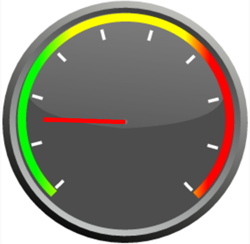
\includegraphics{3Vorgehen/imag/tachometer_mit_nadel.png}
    \caption{Tachometer mit animierter Nadel}
	\label{tachometer_mit_nadel} 
\end{figure}

\subsection{Modularer Aufbau}

Die Applikationsentwicklung basiert auf einer modularen Struktur.  Dadurch wird eine Weiterentwicklung der Applikation ohne Probleme möglich. Ebenfalls wurde beachtet, dass die Applikation sogar in andere Sprachen übersetzt werden können muss, dafür wurden alle Texte, die ersichtlich sind, in einem File aufgenommen und können zentral abgeändert werden, ohne einen Eingriff in den aktuellen Code.






